\section{Multi-Robot Approach for Weld Cost Minimization}

In the approach section(cite section) we discussed how introduction of another robot can increase the number of degrees of freedom and hence allow the robot to perform more complex manipulations. Increasing the degree of complexity of motion can allow us to implement better optimization as well as solve the problems of unreachability and singularity. In this chapter we will discuss the integration of a 2 degrees of freedom rotary table into the existing architecture and how that is utilized to optimize the welding task. 

\subsection{Modeling the Rotary Table}
The existing implementation only contained kinematic description of the 6 axis manipulator with the weld tool tip. In the following subsections, we present a model of the 2 degree of freedom rotary table, along with the kinematic description and present the improved architectural model.
\subsubsection{Architecture of RobotKit}
The following architectural diagram(\ref{fig:img9}) has been color coded for better understanding. Blue represents the core functionalities of RobotKit. Red represents the kinematics and visualization models on which the improvements are implemented. Green represents external configuration files that are loaded inside RobotKit. Yellow represents the OMPL based planning library and pink represents the user interface block. \\
In the existing architecture the Kernel block creates instances of the kinematics and visualization models of the 6 Dof robot, which update the simulation environment based on the data input from the Information Exchange Pipeline. The planner interface class takes input from the kernel and the information exchange pipeline and user input for welding task. It then creates a planning problem and sends it to the OMPL based planning library. The communication between the planner interface and the planning library takes place using dll files. The project configuration file loads information about the dH parameters of the robot, position of the work piece and other relevant objects and in the weld cell. 

\begin{figure}[!htbp] %  figure placement: here, top, bottom, or page
 \centering
   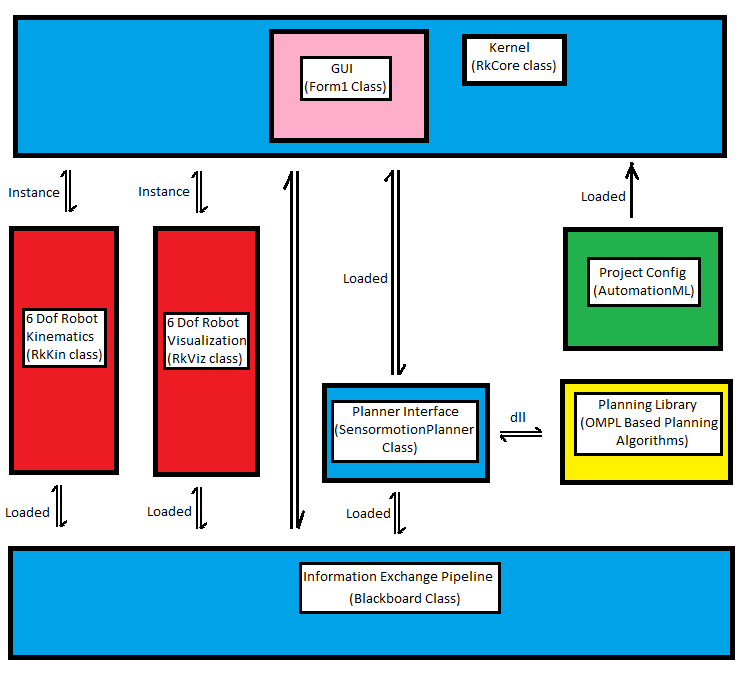
\includegraphics[width=9cm]{images/Original_arch.png}
   \caption[Exisitng Architecture of RobotKit(cite rk)]
   {Exisitng Architecture of RobotKit}  
\label{fig:img9}
\end{figure}

In the following architecture diagram (\ref{fig:img10}) the exact blocks which have been updated are highlighted. The kinematic and the visualization models now also includes definition of rotary table. The project configuration file (highlighted in green) has also been updated to include the dH parameters of the rotary table. 
\begin{figure}[!htbp] %  figure placement: here, top, bottom, or page
 \centering
   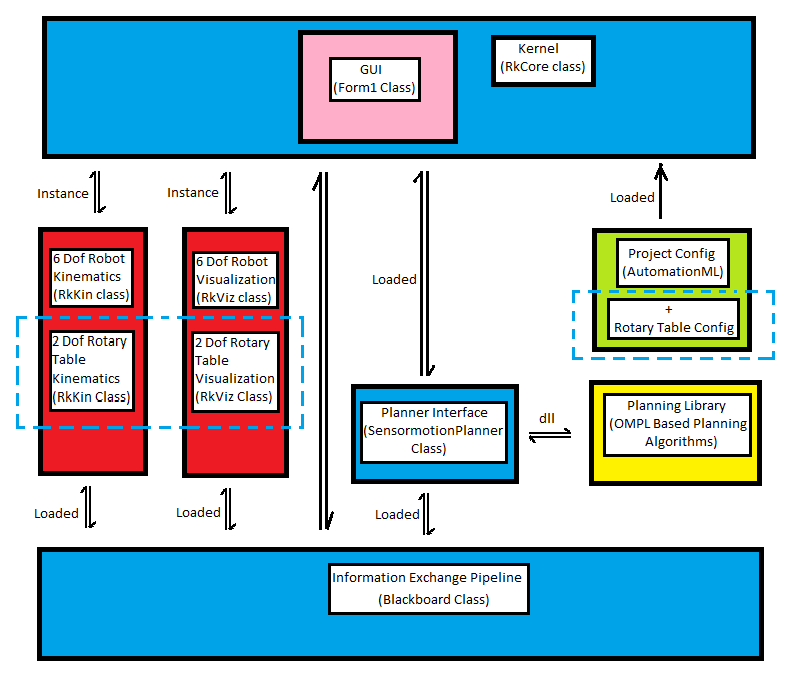
\includegraphics[width=9cm]{images/new_arch.png}
   \caption[Updated Architecture of RobotKit(cite rk)]
   {Updated Architecture of RobotKit}  
\label{fig:img10}
\end{figure}
 

\subsubsection{Generating 3D Models for Simulation}
In order to update the simulation environment, 3D CAD models of the rotary table were created using Solidworks software(cite solidworks), based on the data-sheet specifications. In order to make the simulation mimic the real functioning of the rotary table, the table was divided into 3 separate CAD objects; base, middle joint and top plate. The images for the same are presented herewith. 

\begin{figure}[!htbp] %  figure placement: here, top, bottom, or page
\begin{subfigure}{\linewidth}
   \frame{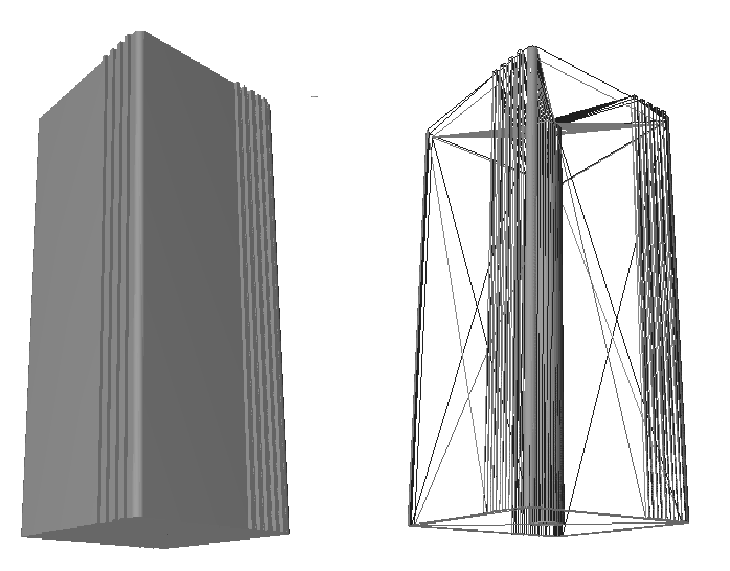
\includegraphics[width=.5\linewidth]{images/Base.png}}
   \frame{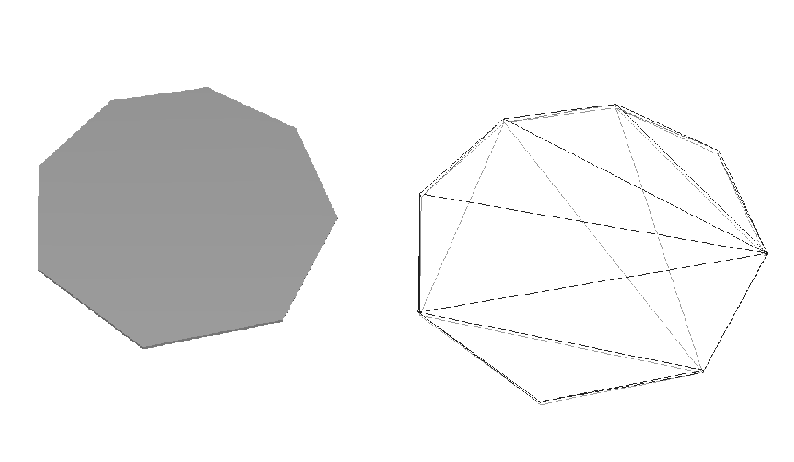
\includegraphics[width=.5\linewidth]{images/Top.png}}
      \caption[dd]{Base and Top Joint models}
   \end{subfigure}\par\medskip
   \begin{subfigure}{\linewidth}
   \centering
   \frame{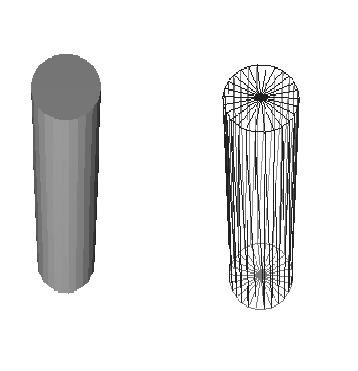
\includegraphics[width=.5\linewidth]{images/Mid.png}}
   \caption[dd]{Middle Joint model}
   \end{subfigure}
\caption[dd]{CAD models of the Rotary Table: Base, Middle and Top}
\label{fig:img11}
\end{figure}
 

\subsubsection{Kinematic Description of the Rotary Table}

The kinematic description of the 2 Dof Rotary table was created using the standard DH parameter approach. The DH parameters as specified in the Reis welding cell data-sheet(cite datasheet) are presented in the following table \ref{tab2}
\begin{table}[!htbp]
\centering
\scalebox{1.2}{%
\frame{\begin{tabular}{@{}lllll@{}}
\toprule
i & $\alpha_{i-1}$ & a\_\{i-1\} & d\_\{i\} & $\theta_{i}$ \\ \midrule
1 & 0              & 0          & 0        & $\theta_{1}$ \\
2 & -90            & 0          & 150 mm     & $\theta_{2}$
\end{tabular}%
}}
\caption{DH parameter of Rotary Table}
\label{tab2}
\end{table}
\\
The next step is to construct the link frames of the joints of the table in accordance with the approach mentioned in (cite Introduction to robotics, jacob book). The frames were plotted in Cartesian space with actual values from the real robot system. The values are the actual coordinates of the joint with respect to the global coordinate frame. Since the rotary table present in the welding cell has 2 Dof, we take Joint 0 as a reference frame, which coincides with the frame of Joint 1. According to the Reis welding cell data-sheet(use cite doc), the axis of rotation of Joint 1 of the rotary table is same as the X axis of the robot frame of the 6 dof manipulator and the axis of rotation of Joint 2 is same as the Z axis of the robot frame of the 6 dof manipulator. \\
In the following figure \ref{fig:img12} the world and robot frames along with the joint frames of the rotary table in the Cartesian coordinate frame are plotted. 
\begin{figure}[!htbp] %  figure placement: here, top, bottom, or page
 \centering
   \frame{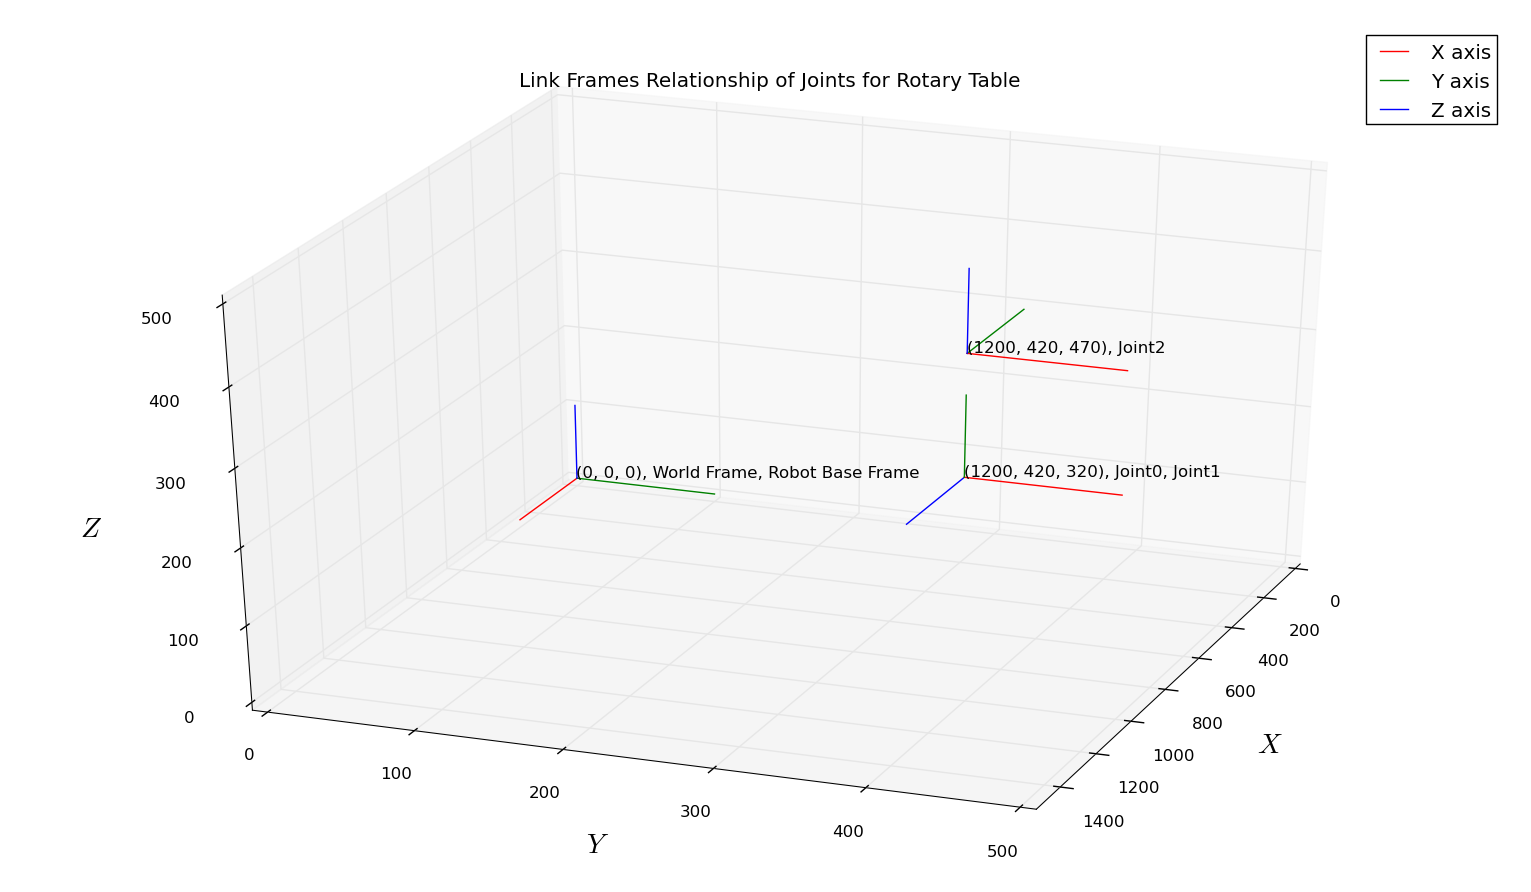
\includegraphics[width=12cm]{images/Frames_jnttab.png}}
   \caption{Link Frame Relationship of Joints of Rotary Table}  
\label{fig:img12}
\end{figure}

Based on the DH parameters from table \ref{tab2} we now construct the forward kinematic chain. 
\begin{equation}
\label{eq20}
_{0}^{1}\textrm{T} = \begin{bmatrix} \cos\theta_{i} & -\sin \theta_{i} & 0 & 0\\ \sin \theta_{i} & \cos \theta_{i} & 0 & 0\\ 0 & 0 & 1 & 0\\ 0 & 0 & 0 & 1 \end{bmatrix}
\end{equation}

\begin{equation}
\label{eq21}
_{2}^{1}\textrm{T} = \begin{bmatrix} \cos\theta_{i} & -\sin \theta_{i} & 0 & 0\\ 0 & 0 & 1 & 150\\ -\sin \theta_{i} & -\cos\theta_{i} & 0 & 0\\ 0 & 0 & 0 & 1 \end{bmatrix}
\end{equation}

\begin{equation}
\label{eq22}
\textrm{T}_{table} =_{2}^{0}\textrm{T}_{1}^{0}\textrm{T}._{2}^{1}\textrm{T} = \begin{bmatrix} \cos^{2}\theta_{i}& -\cos\theta_{i}.\sin\theta_{i} & -\sin\theta_{i} & -150*\sin\theta_{i}\\ \cos\theta_{i}.\sin\theta_{i} & -\sin^{2}\theta_{i} & \cos\theta_{i} & 150*\cos\theta_{i}\\ -\sin\theta_{i} & -\cos\theta_{i}& 0 & 0\\ 0& 0& 0& 1\end{bmatrix}
\end{equation}

\subsubsection{Workpiece Transformation}

Since the main objective of moving the rotary table is to move the work piece, a transformation function is also necessary to simulate the changed position of the work piece in accordance with the motion of the table. 

\begin{algorithm}[!htbp]
	\caption{Transformation of Work Piece position wrt Table Position}
	\label{algo2}
	\textbf{Given:} $ \text{Original }(\textit{$_{T}^{W}P$}, \textit{$_{T}^{W}O$})\text{pose and orientation information}  \bigwedge \text{ new}\\(\textit{$_{T}^{W}P_{new}$}, \textit{$_{T}^{W}O_{new}$}) \text{pose and orientation information} \text{ of table wrt. to world frame }\\ \text{ and current position and orientation } (\textit{$_{WP}^{W}P$}, \textit{$_{WP}^{W}O$}) \text{information of work piece wrt.} \\ \text{world frame} $ \\ \\
	\textbf{Output:} $\text{New}(\textit{$_{WP}^{W}P_{new}$},\textit{$_{WP}^{W}O_{new}$}) \text{position and orientation  information} \\ \text{of work piece wrt. world frame}$\\
	
	\begin{algorithmic}[1]
		\State $\textit{$_{T}^{W}T$} \gets Converttomatrix(\textit{$_{T}^{W}P$},\textit{$_{T}^{W}O$})$
		\State $\textit{$_{WP}^{W}P$} \gets Converttomatrix(\textit{$_{WP}^{W}P$},\textit{$_{WP}^{W}O$})$
		\State $\textit{$_{T}^{W}T_{new}$} \gets Converttomatrix(\textit{$_{T}^{W}P_{new}$}, \textit{$_{T}^{W}O_{new}$})$ \\
		\If{[${Initializing program}$]}
		\State $\textit{$_{WP}^{T}T_{ref}$} \gets \textit{$_{T}^{W}T^{-1}$} * \textit{$_{WP}^{W}T$}$
		\EndIf \\
		\If{[$\text{user offset work piece position}$]}
		\State $\textit{$_{WP}^{T}T^{'}$} \gets \textit{$_{T}^{W}T^{-1}$} * \textit{$_{WP}^{W}T^{'}$}$
		\State $\textit{$_{WP}^{T}T_{ref}$} \gets $\textit{$_{WP}^{T}T^{'}$}
		\EndIf \\
		
		\State $\textit{$_{WP}^{W}T_{new}$} \gets \textit{$_{T}^{W}T_{new}^{-1}$} * \textit{$_{WP}^{T}T_{ref}$}$\\
		\State $\textit{$_{WP}^{W}P_{new}$} \gets position(\textit{$_{WP}^{W}T_{new}$})$
		\State $\textit{$_{WP}^{W}O_{new}$} \gets matrixtoeulerangles(\textit{$_{WP}^{W}T_{new}$})$\\
		\If{[$Edge to be welded selected$]}
		\State $SelectedEdgeTransform()$
		\EndIf \\
		\textbf{return:} $\textit{$_{WP}^{W}P_{new}$},\textit{$_{WP}^{W}O_{new}$}$
	\end{algorithmic}
\end{algorithm}
\newpage
\subsubsection{Selected Edge Transformation}

\begin{algorithm}
	\caption{Transformation of Selected Edge wrt Work Piece Position}
	\label{algo3}
	\textbf{Given:} $ \text{Original pose and orientation information of start(\textit{$_{SP}^{W}P$}, \textit{$_{SP}^{W}O$}) and goal} \\ \text{points(\textit{$_{GP}^{W}P$}, \textit{$_{GP}^{W}O$}) }  \bigwedge \text{ new}(\textit{$_{WP}^{W}P_{new}$}, \textit{$_{WP}^{W}O_{new}$}) \text{pose and orientation information} \\ \text{ of work piece wrt. to world frame } \text{ and old position and orientation }\\ (\textit{$_{WP}^{W}P$}, \textit{$_{WP}^{W}O$}) \text{information of work piece wrt. world frame} $ \\ 
	\textbf{Output:} $\text{New pose and orientation information of start(\textit{$_{SP}^{W}P_{new}$}, \textit{$_{SP}^{W}O_{new}$}) and } \\ \text{goal points(\textit{$_{GP}^{W}P_{new}$}, \textit{$_{GP}^{W}O_{new}$}) }$\\
	
	\begin{algorithmic}[1]
		\State $\textit{$_{SP}^{W}T$} \gets Converttomatrix(\textit{$_{SP}^{W}P$},\textit{$_{SP}^{W}O$})$
		\State $\textit{$_{GP}^{W}T$} \gets Converttomatrix(\textit{$_{GP}^{W}P$},\textit{$_{GP}^{W}O$})$
		\State $\textit{$_{WP}^{W}T$} \gets Converttomatrix(\textit{$_{WP}^{W}P$},\textit{$_{WP}^{W}O$})$
		\State $\textit{$_{WP}^{W}T_{new}$} \gets Converttomatrix(\textit{$_{WP}^{W}P_{new}$}, \textit{$_{WP}^{W}O_{new}$})$ 
		\For{[$each selected edge$]} 
		\If{[${Initializing program}$]}
		\State $\textit{$_{SP}^{WP}T_{ref}$} \gets \textit{$_{WP}^{W}T^{-1}$} * \textit{$_{SP}^{W}T$}$
		\State $\textit{$_{GP}^{WP}T_{ref}$} \gets \textit{$_{WP}^{W}T^{-1}$} * \textit{$_{GP}^{W}T$}$
		\EndIf 
		\If{[$\text{user offset work piece position}$]}
		\State $\textit{$_{SP}^{WP}T^{'}$} \gets \textit{$_{WP}^{W}T_{new}^{-1}$} * \textit{$_{SP}^{W}T$}$
		\State $\textit{$_{GP}^{WP}T^{'}$} \gets \textit{$_{WP}^{W}T_{new}^{-1}$} * \textit{$_{GP}^{W}T$}$
		\State $\textit{$_{SP}^{WP}T_{ref}$} \gets $\textit{$_{SP}^{WP}T^{'}$}
		\State $\textit{$_{GP}^{WP}T_{ref}$} \gets $\textit{$_{SP}^{WP}T^{'}$}
		\EndIf 		
		\State $\textit{$_{SP}^{W}T_{new}$} \gets \textit{$_{WP}^{W}T_{new}^{-1}$} * \textit{$_{SP}^{WP}T_{ref}$}$
		\State $\textit{$_{GP}^{W}T_{new}$} \gets \textit{$_{WP}^{W}T_{new}^{-1}$} * \textit{$_{GP}^{WP}T_{ref}$}$
		
		\State $\textit{$_{SP}^{W}P_{new}$} \gets position(\textit{$_{SP}^{W}T_{new}$})$
		\State $\textit{$_{SP}^{W}O_{new}$} \gets matrixtoeulerangles(\textit{$_{SP}^{W}T_{new}$})$
		\State $\textit{$_{GP}^{W}P_{new}$} \gets position(\textit{$_{GP}^{W}T_{new}$})$
		\State $\textit{$_{GP}^{W}O_{new}$} \gets matrixtoeulerangles(\textit{$_{GP}^{W}T_{new}$})$\\
		
		\EndFor \\
		\textbf{return:} $\textit{$_{SP}^{W}P_{new}$},\textit{$_{SP}^{W}O_{new}$},\textit{$_{GP}^{W}P_{new}$},\textit{$_{GP}^{W}O_{new}$}$
	\end{algorithmic}
\end{algorithm}
\newpage
\subsection{Cost Function Formulation}
\label{ssec:cst}
Two different cost functions were formulated and finally a weighted combination of the two was created, to form the final cost function. The plots of the cost functions were created by running the planner for every different orientations of the table for the following two work pieces. For each workpiece 2 edges were randomly selected to demonstrate the behaviors based on the cost function definition. The edges also contain the convention definition, which specifies the alignment of the TCP with respect to the selected edge. For example in \ref{fig:imgoridef1} and \ref{fig:imgoridef2}, the TCP moves along the planned path in accordance with the convention; the X axis (marked by red) points from start to goal point along the edge to be welded, and the Y (marked by green) and Z (marked by blue) maintain an angle of 45$^{\circ}$ with respect to the selected edge. \\
\begin{figure}[!htbp] %  figure placement: here, top, bottom, or page
	\centering
	\begin{subfigure}[b]{0.4\textwidth}
		\frame{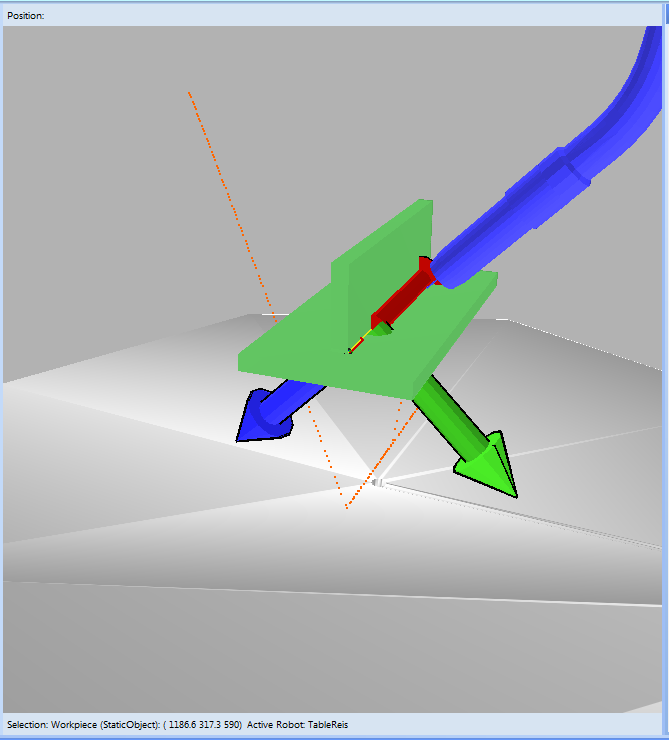
\includegraphics[width=1\textwidth,height=0.2\textheight]{images/tcp_ori.png}}
		\caption{}
		\label{fig:imgoridef1}
	\end{subfigure}
	\begin{subfigure}[b]{0.4\textwidth}
		\frame{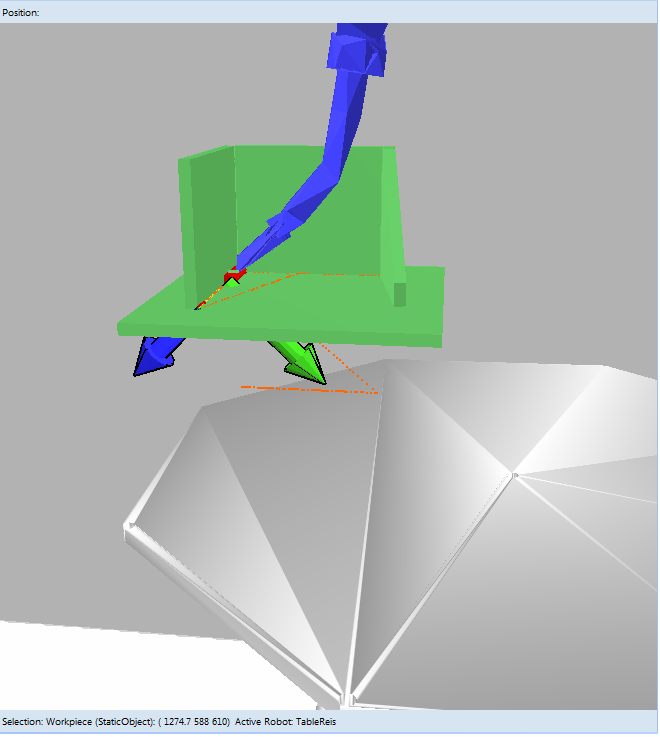
\includegraphics[width=1\textwidth,height=0.2\textheight]{images/tcp_ori_al.png}}
		\caption{} 
		\label{fig:imgoridef2}
	\end{subfigure}	
	\caption{Convention Definition of TCP with Respect  to Weld Edge}  
	\label{fig:tcor}
\end{figure}

\begin{figure}[!htbp] %  figure placement: here, top, bottom, or page	
	\centering
	\begin{subfigure}[b]{0.4\textwidth}	
		 \frame{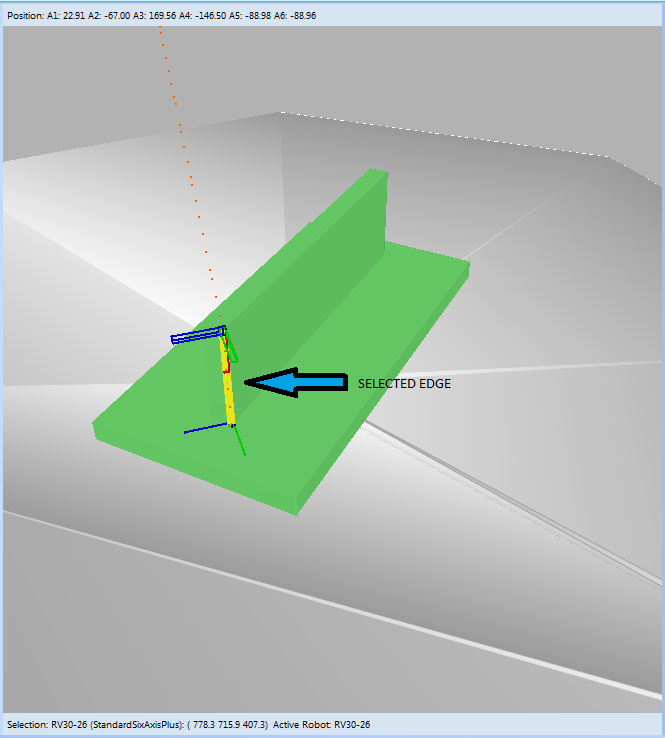
\includegraphics[width=1\textwidth,height=0.2\textheight]{images/normwp_left.png}}
		 \caption{Left Vertical Edge of T-Joint Workpiece}
		\label{fig:imguc1}
	\end{subfigure}
	\begin{subfigure}[b]{0.4\textwidth}		
		\frame{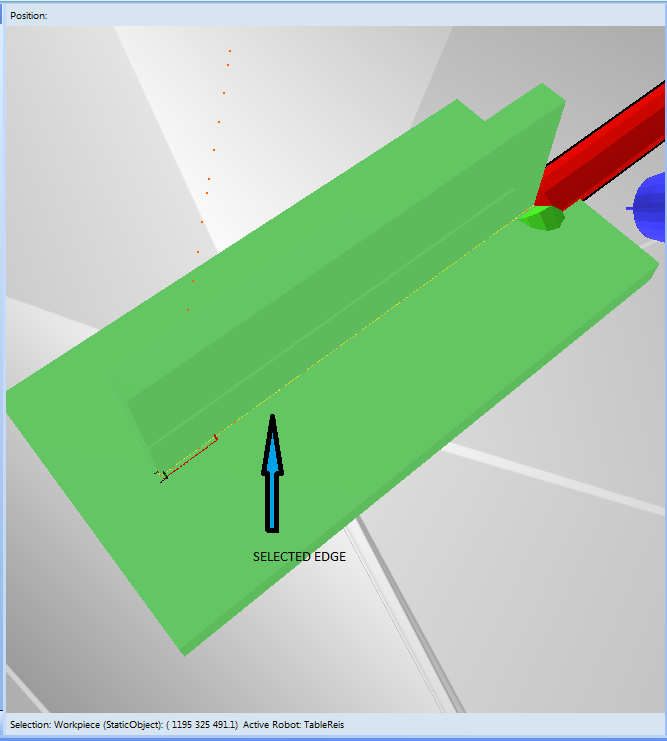
\includegraphics[width=1\textwidth,height=0.2\textheight]{images/normwp_flat.png}}
		\caption{Horizontal Edge of T-Joint Work  piece} 
	\label{fig:imguc2}
	\end{subfigure}		
	\caption{Simple T-Joint Workpiece}  
	\label{fig:uc1}
\end{figure}
\textbf{1st Use Case:}This \ref{fig:uc1} is a T-Jointed work piece for which we select two edges, to demonstrate the two different cost functions. The edges for which weld paths are to be generated are marked by yellow lines and pointed at by the arrows

\textbf{2nd Use Case:}The welding robot was demonstrated in Automatic Messe 2016(Munich) in which this(\ref{fig:uc2}) work piece was used to demonstrate the autonomous program generation for welding. For this workpiece, two edges were considered, which are marked yellow lines and pointed at by the arrows.
\begin{figure}[!htbp] %  figure placement: here, top, bottom, or page
	\centering
	\begin{subfigure}[b]{0.4\textwidth}
		\frame{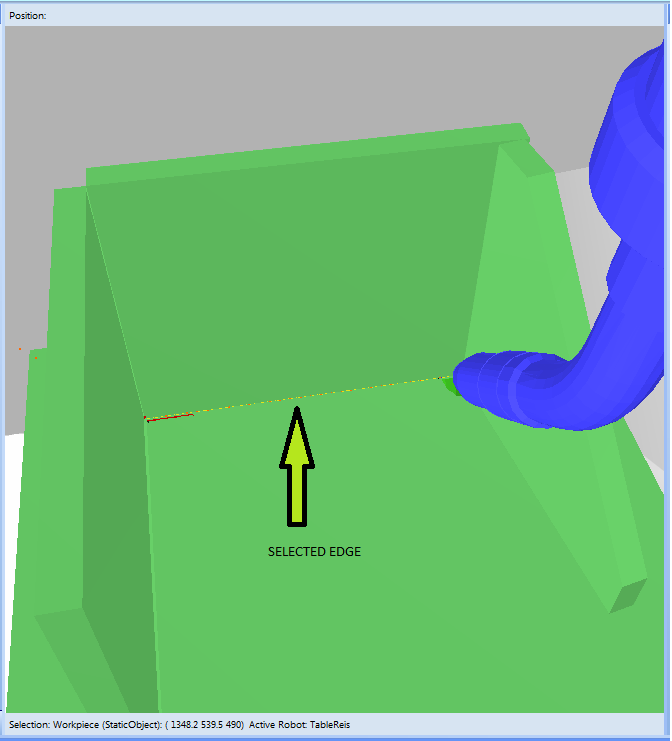
\includegraphics[width=1\textwidth,height=0.2\textheight]{images/auto_flat.png}}
		\caption{Horizontal Edge of Automatica 2016 Workpiece}  
		\label{fig:imguc3}
	\end{subfigure}
	\begin{subfigure}[b]{0.4\textwidth}
		\frame{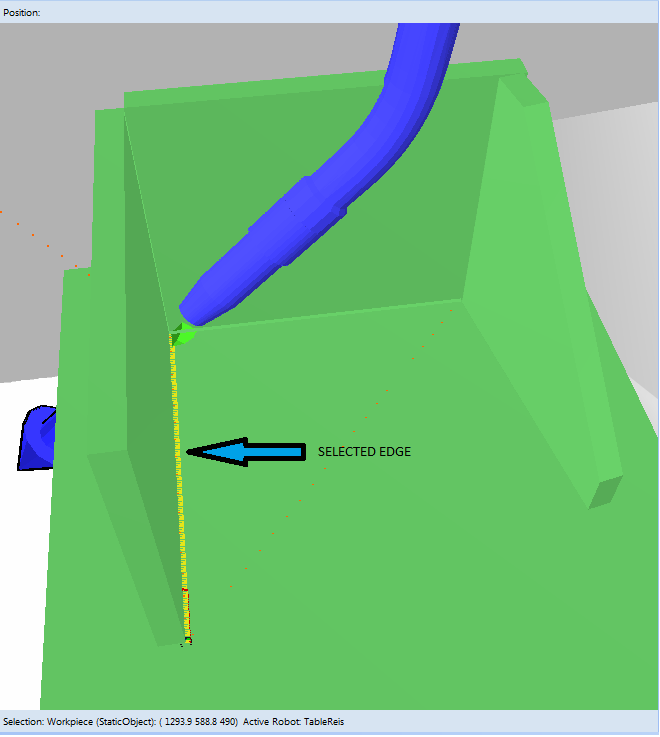
\includegraphics[width=1\textwidth,height=0.2\textheight]{images/auto_left.png}}
		\caption{Inner Left Edge of Automatica 2016 Workpiece}  
		\label{fig:imguc4}
	\end{subfigure}	
\caption{Workpiece used in Automatica 2016 demonstration}
\label{fig:uc2}
\end{figure}

\subsubsection{Difference of TCP orientation and Workpiece edge}
\label{sssec:tcpcst}
In (\ref{fig:tcor}) we saw the relationship between TCP orientation and the workpiece convention. In order to generate high quality weld paths, it is necessary to orient the TCP in accordance with the optimal TCP orientation definition. Therefore for our first cost function definition; we consider the difference between the actual TCP orientation and the optimal welding process defined TCP orientation (cite ppr). The greater the difference, higher the cost and vice-versa. The difference of the quaternions is calculated using the following steps as defined in (cite ppr).
\begin{itemize}
	%content...
	\label{algo4ppr}
	\item Both the sets of quaternions are defined using the standard convention og 4 quaternion components namely: $q1,q2,q3,q4$
	\item Calculate the normal of optimal and actual quaternion values.
	\item Calculate the inverse of the normalized optimal quaternion and multiply with the normalized actual quaternion to obtain the difference of the quaternions.
	\item Convert the difference of the quaternions into an angle value.
	\item Ensure difference angle lies within -180$^{\circ}$ and 180$^{\circ}$
	\item return $C_{tcp}$(\textit{Solution})
\end{itemize}
In order to analyze the cost function, it was necessary to plot the cost values generated for each welding path for various orientation of the table. We considered a range of -80$^{\circ}$ to +80$^{\circ}$ for 1st joint angle and -140$^{\circ}$ to 140$^{\circ}$ for 2nd joint angle of the table. Plots for both use cases; as illustrated in figures \ref{fig:uc1} and \ref{fig:uc2}
were generated.
\begin{figure}[!htbp] %  figure placement: here, top, bottom, or page
	\centering
	\begin{subfigure}[b]{0.4\textwidth}
		\frame{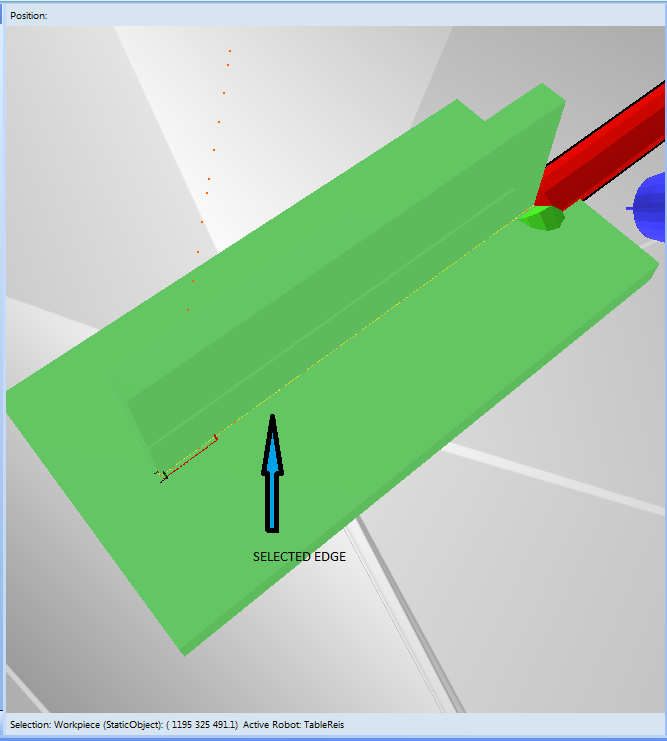
\includegraphics[width=1\textwidth,height=0.2\textheight]{images/normwp_flat.png}}
		\caption{Edge to be welded}  
		\label{fig:cp1b}
	\end{subfigure}
	\begin{subfigure}[b]{0.4\textwidth}
		\frame{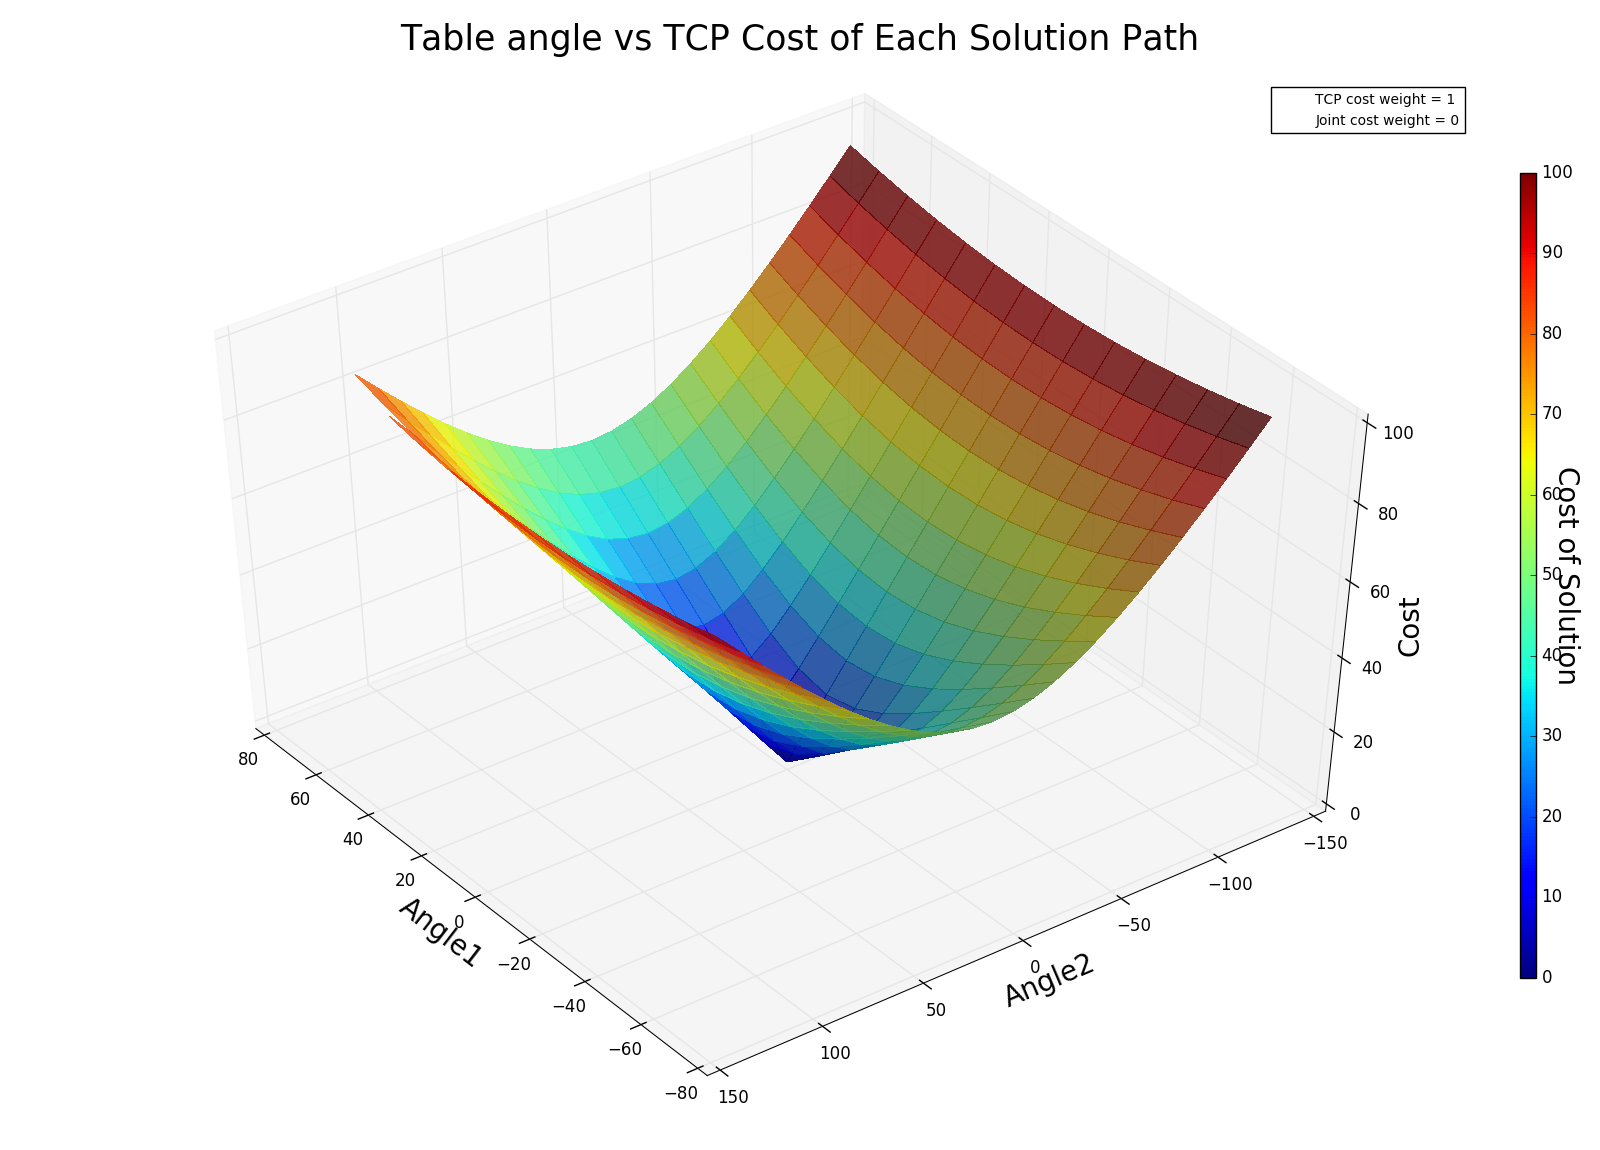
\includegraphics[width=1\textwidth,height=0.2\textheight]{images/orihori_tcpcst.png}}
		\caption{Cost Function Plot}  
	\label{fig:cp1a}
	\end{subfigure}	
	\caption{Cost Function Plot of T-Jointed workpiece: TCP orientation}
	\label{fig:cp1}
\end{figure}
\\
The edge to be welded is marked in yellow \ref{fig:cp1b}. In this cost plot \ref{fig:cp1a}, the minimum cost is obtained when both the joint angles of the table are at 0$^{\circ}$. In the plot, red represents a higher cost region while blue represents lower cost. The cost values were scaled from 0 to 100 to enable us to compare the various results.

\begin{figure}[!htbp] %  figure placement: here, top, bottom, or page
	\centering
	\begin{subfigure}[b]{0.4\textwidth}
		\frame{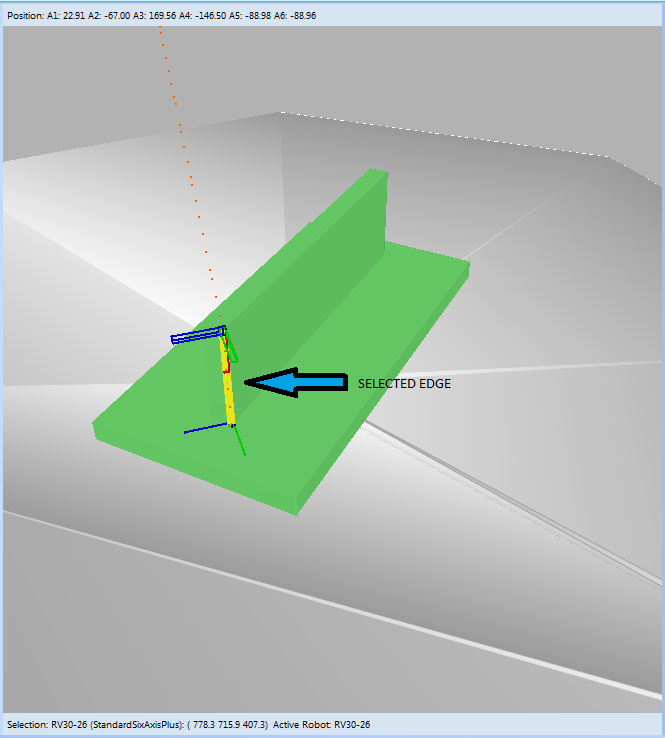
\includegraphics[width=1\textwidth,height=0.2\textheight]{images/normwp_left.png}}
		\caption{Edge to be welded}  
		\label{fig:cp2b}
	\end{subfigure}
	\begin{subfigure}[b]{0.4\textwidth}
		\frame{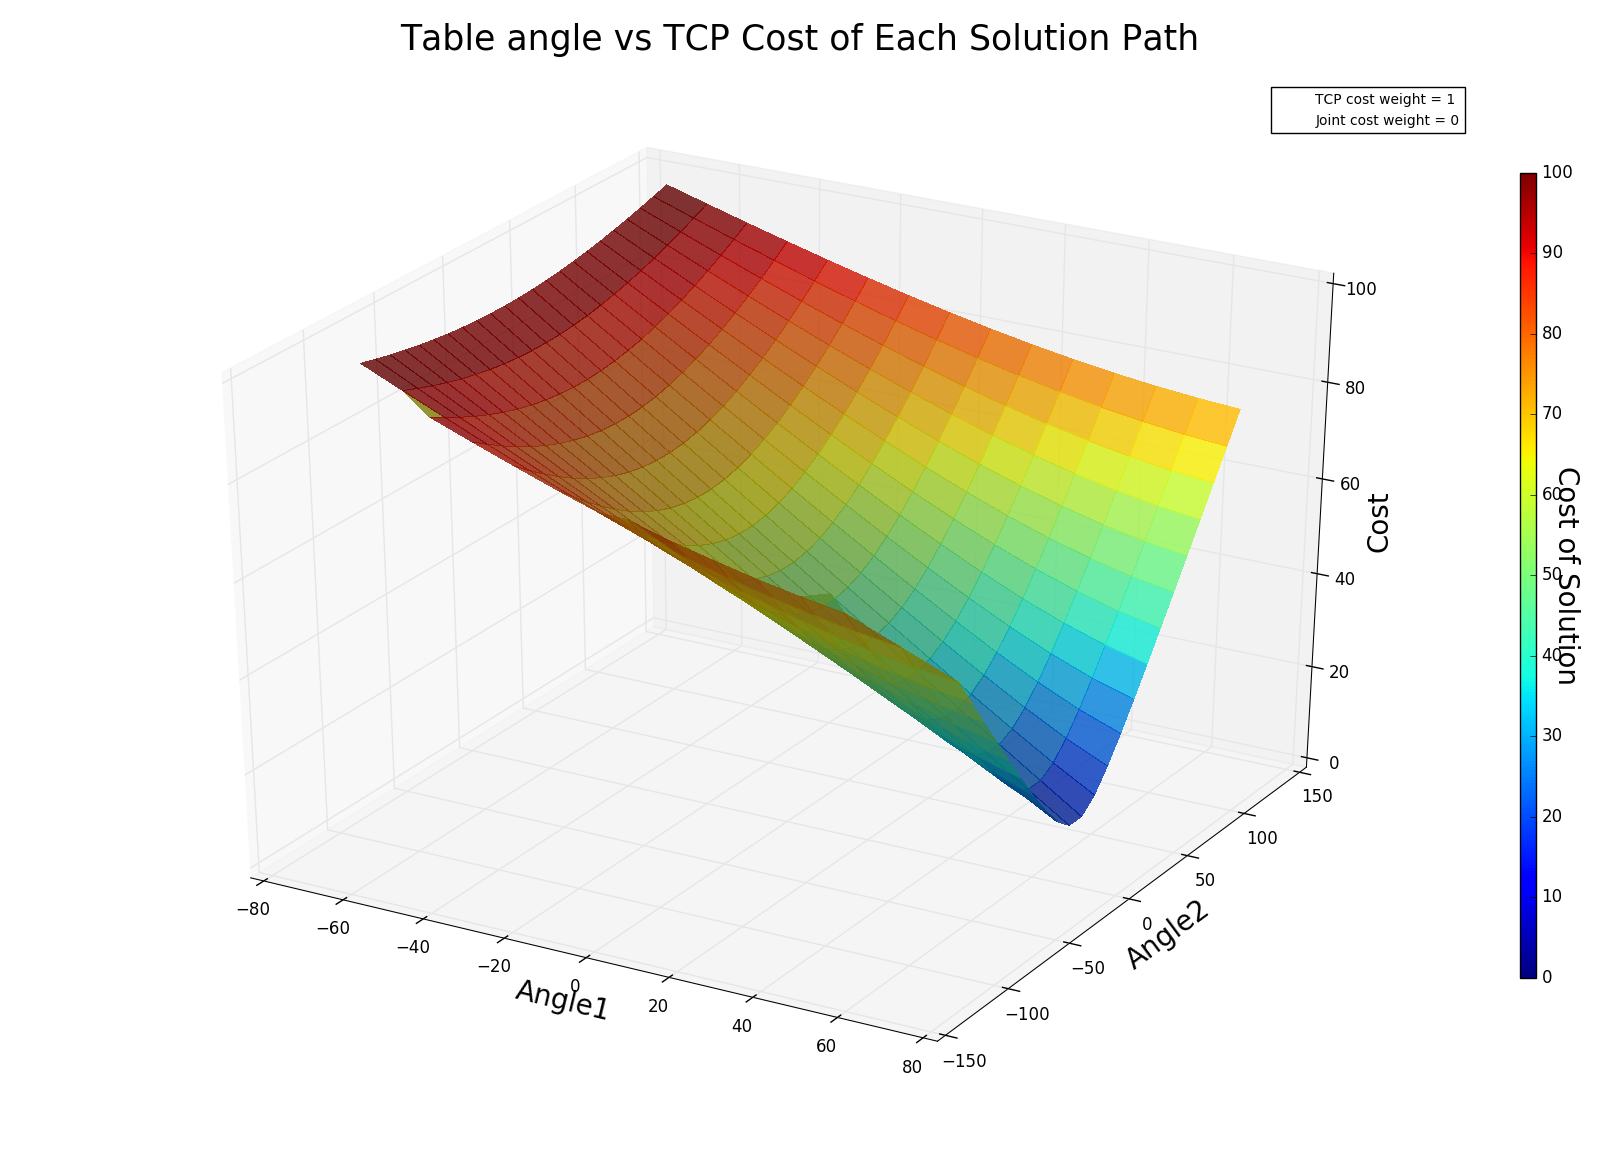
\includegraphics[width=1\textwidth,height=0.2\textheight]{images/orileft_tcpcst.png}}
		\caption{Cost Function Plot}  
		\label{fig:cp2a}
	\end{subfigure}	
	\caption{Cost Function Plot of T-Jointed workpiece: TCP orientation}
	\label{fig:cp2}
\end{figure}
The edge to be welded is marked in yellow\ref{fig:cp2b}. In the cost plot \ref{fig:cp2a}, the minimum cost is obtained when the joint angle - which moves the table along x axis - is at +80$^{\circ}$ and joint angle 2 - rotation along Z axis - is at 0$^{\circ}$.
\clearpage
The cost functions for the Automatica 2016 workpiece are presented below. Similar to the previous cases, the edge to be welded is marked in yellow. Red represents a higher cost gradient while blue represents a lower one. The cost value was scaled in a range of 0 to 100 to make it easier to compare the results.

\begin{figure}[!htbp] %  figure placement: here, top, bottom, or page
	\centering
	\begin{subfigure}[b]{0.4\textwidth}
		\frame{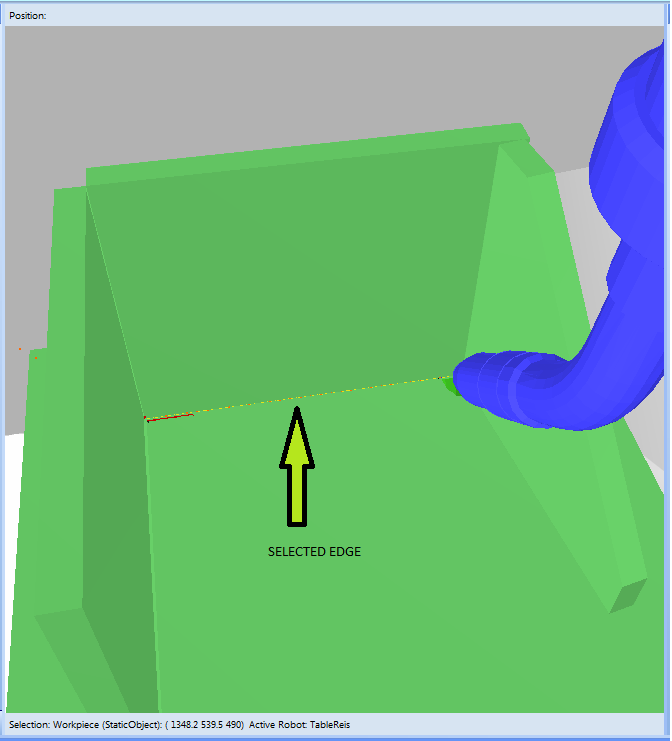
\includegraphics[width=1\textwidth,height=0.2\textheight]{images/auto_flat.png}}
		\caption{Edge to be welded}  
		\label{fig:cp3b}
	\end{subfigure}
	\begin{subfigure}[b]{0.4\textwidth}
		\frame{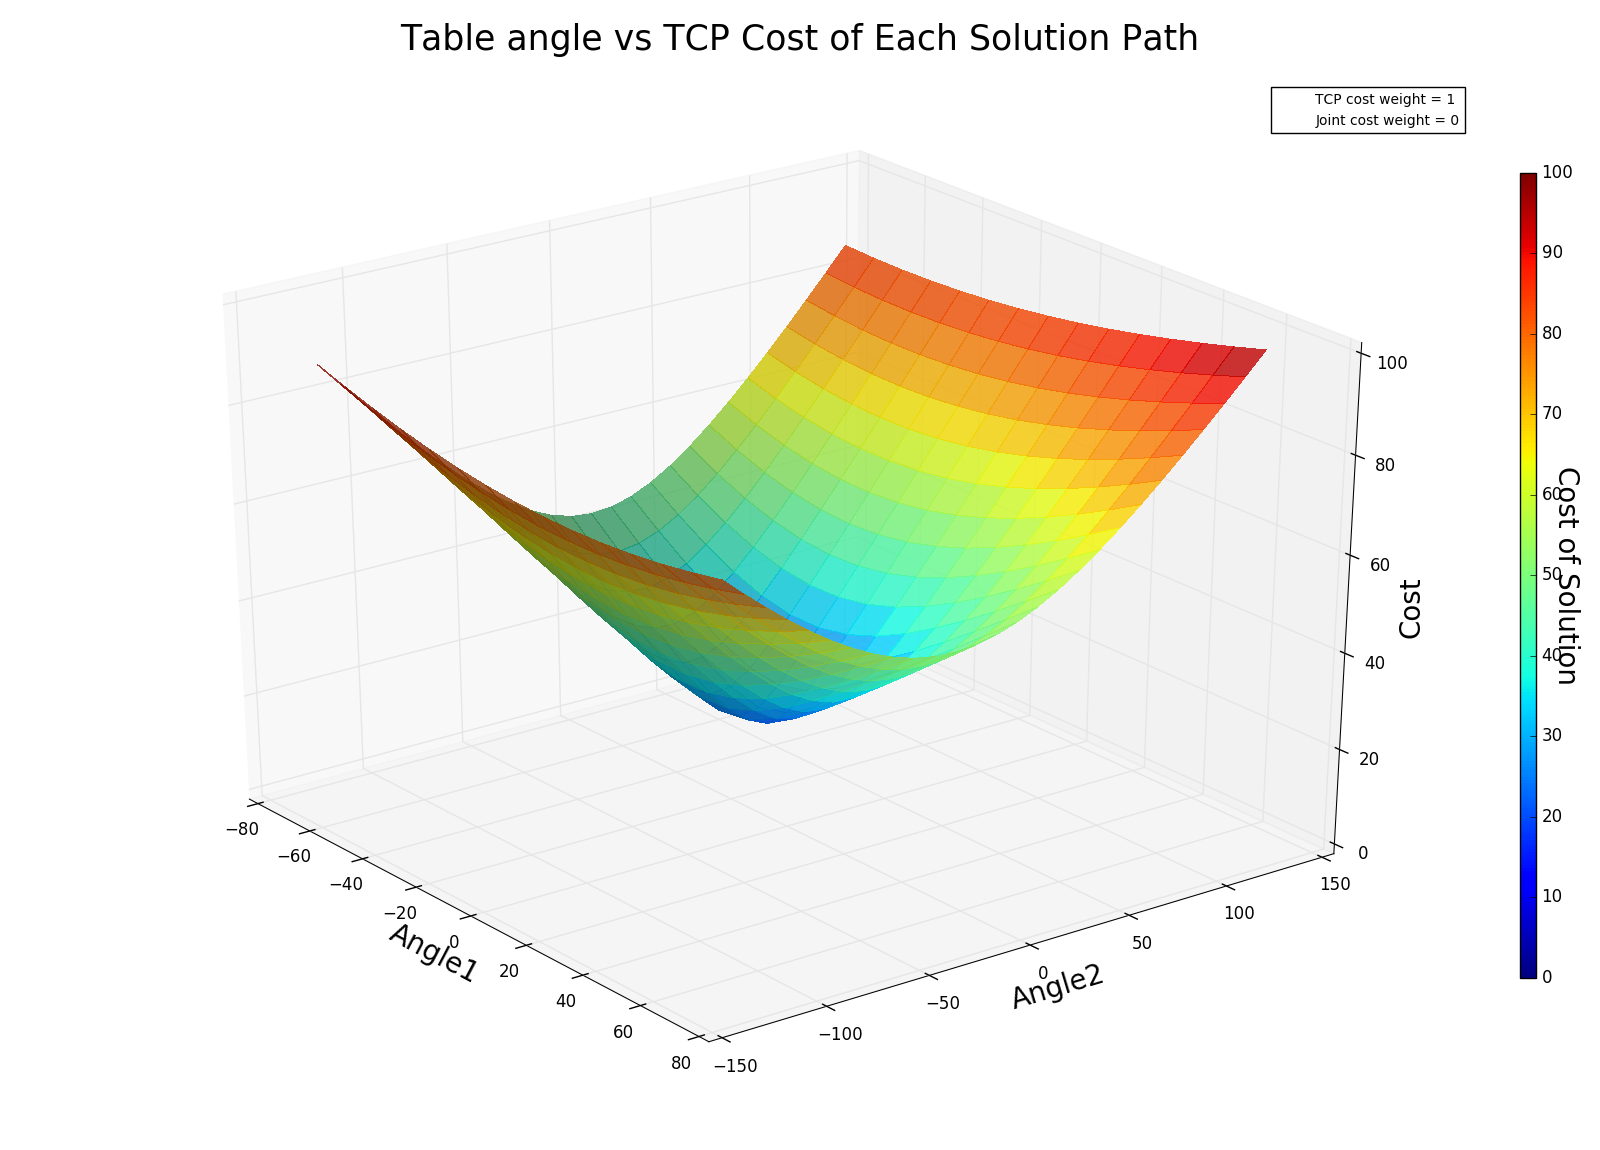
\includegraphics[width=1\textwidth,height=0.2\textheight]{images/autohori_tcpcst.png}}
		\caption{Cost Function Plot}  
		\label{fig:cp3a}
	\end{subfigure}	
	\caption{Cost Function Plot of Automatica workpiece: TCP orientation}
	\label{fig:cp3}
\end{figure}
For this particular weld task, there is a collision at both the start and end points of the weld path between the TCP and workpiece. For this reason the TCP is rotated by certain degrees at both the start and end point, which results in the minimum cost to be high compared to \ref{fig:cp1a}, even though the weld paths are quite similar. The collision scenario is illustrated in \ref{fig:coll}
\begin{figure}[!htbp] %  figure placement: here, top, bottom, or page
	\centering
	\begin{subfigure}[b]{0.4\textwidth}
		\frame{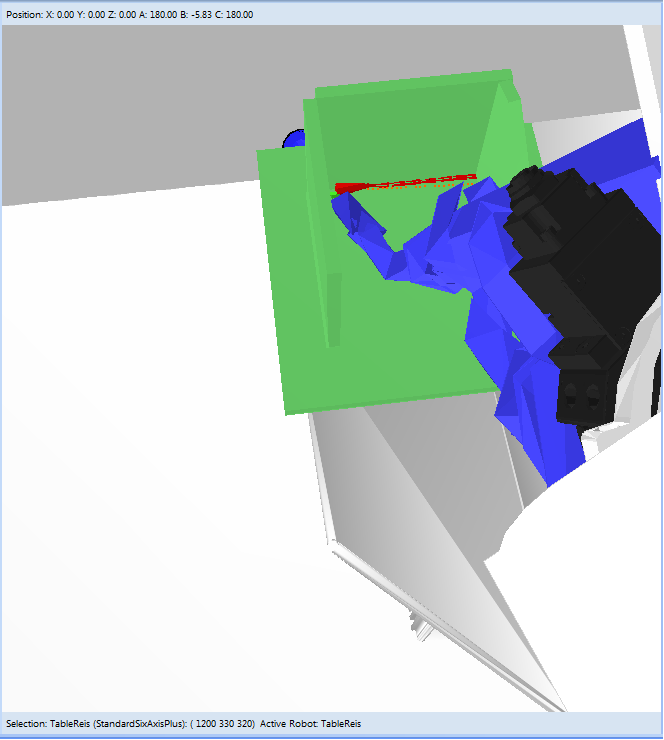
\includegraphics[width=1\textwidth,height=0.2\textheight]{images/auto_strtc.png}}
		\caption{Collision at Start Point}  
		\label{fig:colls}
	\end{subfigure}
	\begin{subfigure}[b]{0.4\textwidth}
		\frame{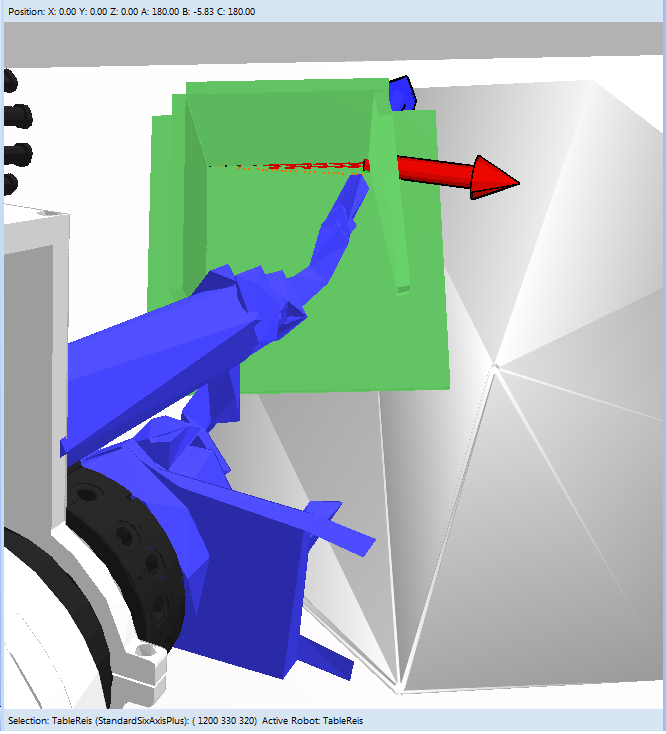
\includegraphics[width=1\textwidth,height=0.2\textheight]{images/auto_endc.png}}
		\caption{Collision at End Point}  
		\label{fig:collg}
	\end{subfigure}	
	\caption{Collision of TCP with workpiece}
	\label{fig:coll}
\end{figure}\\
For the use case in figure:\ref{fig:cp4}, the minimum cost can be observed from \ref{fig:cp4a}, to be when joint angle 1 is at 0$^{\circ}$ and joint angle 2 is at 90$^{\circ}$. Similar to the situation described in (\ref{fig:coll}), a collision at the end point of the selected edge, results in the minimum cost to become significantly high.
\begin{figure}[!htbp] %  figure placement: here, top, bottom, or page
	\centering
	\begin{subfigure}[b]{0.4\textwidth}
		\frame{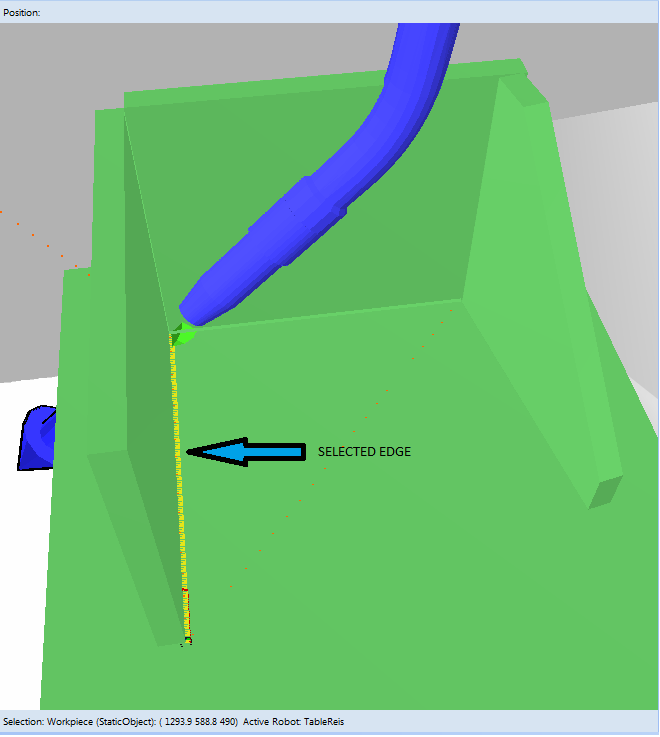
\includegraphics[width=1\textwidth,height=0.2\textheight]{images/auto_left.png}}
		\caption{Edge to be welded}  
		\label{fig:cp4b}
	\end{subfigure}
	\begin{subfigure}[b]{0.4\textwidth}
		\frame{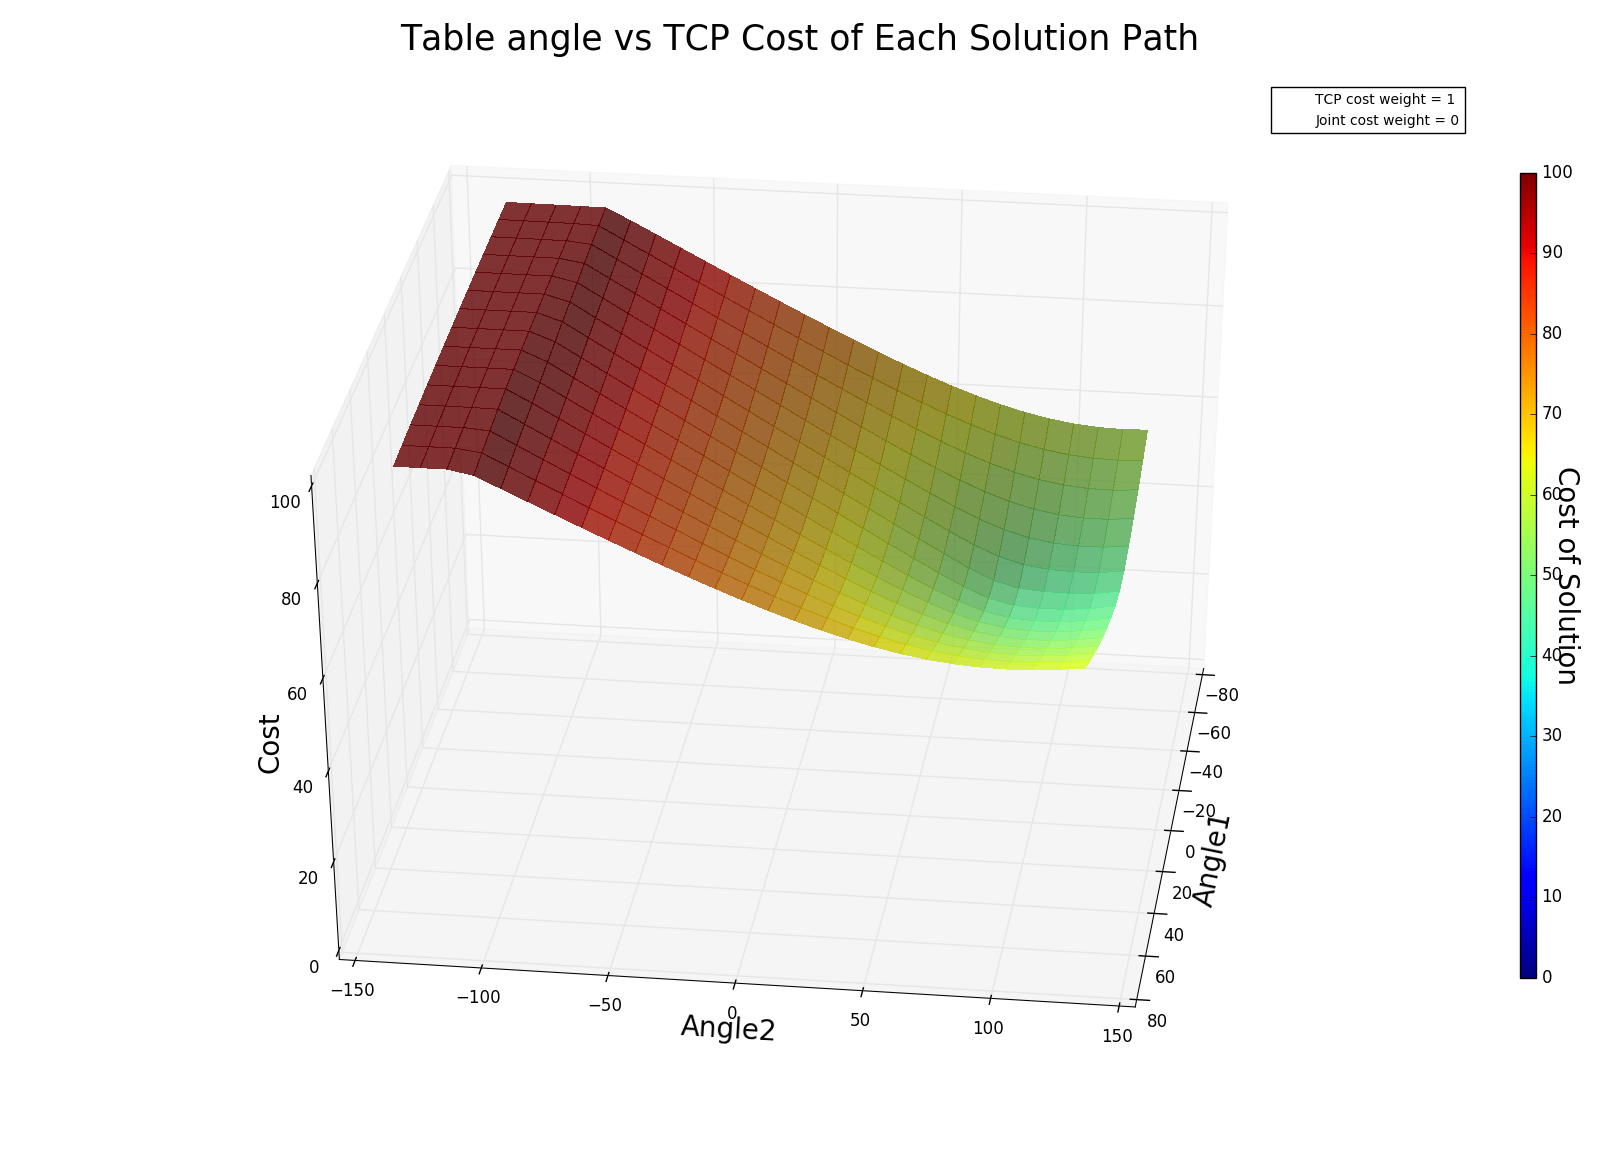
\includegraphics[width=1\textwidth,height=0.2\textheight]{images/autolft_tcpcst.png}}
		\caption{Cost Function Plot}  
		\label{fig:cp4a}
	\end{subfigure}	
	\caption{Cost Function Plot of Automatica workpiece: TCP orientation}
	\label{fig:cp4}
\end{figure}

\subsubsection{Cost Function based on Joint Movement}
\label{sssec:jntcst}
Industrial robots usually carry heavy load which makes it necessary to use high powered motors to move the bigger joints like the 1st and 2nd joints. However, usually for the smaller joints i.e. 4,5 and 6 lower powered motors are used as the load carried by these joints are lower. This concept was exploited to formulate a cost function, wherein the goal is to find weld path plans for which the movement of the bigger joints are minimal. The following table(\ref{tab3}) illustrates the power consumption of the motors of the 6 joints for the Reis Robot. 
\begin{table}[!ht]
	\centering
	\caption{Reis Robot Joint Specifications}
	\label{tab3}
	\begin{tabular}{@{}cccccc@{}}
		\toprule
		& Voltage(V) & Current(A) & Power(kW) & Torque(Nm) & RPM  \\ \midrule
		Base Joint(M1)  & 360        & 10         & 3.6       & 12         & 3800 \\
		2nd Joint(M2)   & 360        & 16.2       & 4.9       & 21.5       & 3800 \\
		3rd Joint(M3)   & 360        & 7.7        & 2.7       & 10.5       & 3800 \\
		4th Joint(M4)   & 360        & 5.1        & 1.9       & 6.2        & 3800 \\
		5th Joint(M5)   & 360        & 5.1        & 1.9       & 6.2        & 3800 \\
		Wrist Joint(M6) & 360        & 2.4        & 0.8       & 2.7        & 4000 \\ \bottomrule
	\end{tabular}
\end{table}
The first step for plotting the space, was to generate weld path solutions for every possible values of the table joint angles and record the corresponding joint angle values of robot. The joint angle values were recorded for all solution points of each weld path along with the start and goal points. Next, to calculate the cost value, we take the weighted sum of the amount of joint movement for the a particular solution path. Total joint movement is the sum of  difference of the joint angles between two consecutive solution points of a solution path. In \ref{eq23}, $C_{final}$ represents the joint cost, $w_{i}$ represents weightage value of joint \textit{i}, $\theta$ is the angle value of joint \textit{i} in degrees, \textit{k} is the solution point number and \textit{n} is the maximum number of solution points generated for a particular edge.
\begin{equation}
\label{eq23}
C_{joint}(\textit{Solution}) = \sum_{i=1}^{6}(w_{i}*\sum_{k=1}^{n}\Delta \theta_{i,k})
\end{equation}
where,
\begin{equation}
\label{eq24}
\Delta \theta_{i,k} = \theta_{i,k+1} - \theta_{i,k}
\end{equation}

The cost value was scaled in a range of 0 to 100 similar to \hyperref[sssec:tcpcst]{previous section} in order to maintain uniformity and allow us to compare the results, we will next analyze the cost functions plots.

\begin{figure}[!ht] %  figure placement: here, top, bottom, or page
	\centering
	\begin{subfigure}[b]{0.4\textwidth}
		\frame{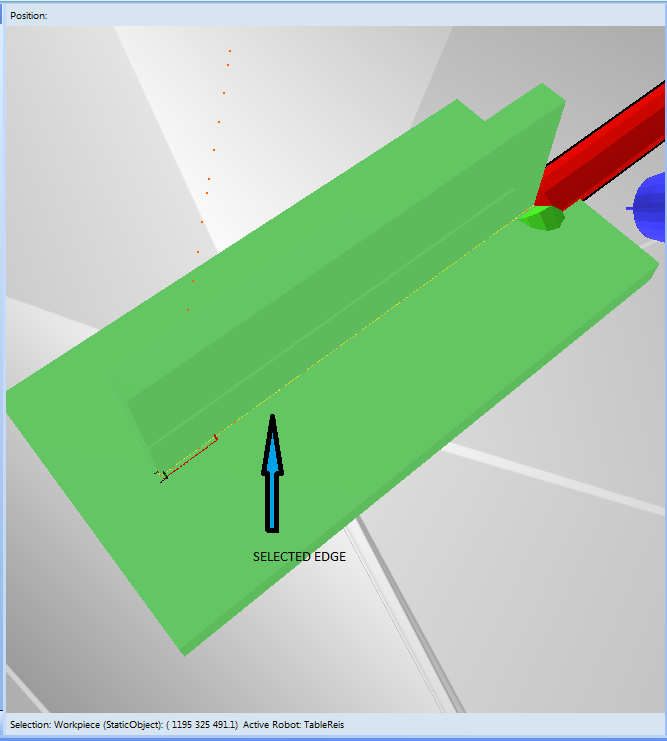
\includegraphics[width=1\textwidth,height=0.2\textheight]{images/normwp_flat.png}}
		\caption{Edge to be welded}  
		\label{fig:17a}
	\end{subfigure}
	\begin{subfigure}[b]{0.4\textwidth}
		\frame{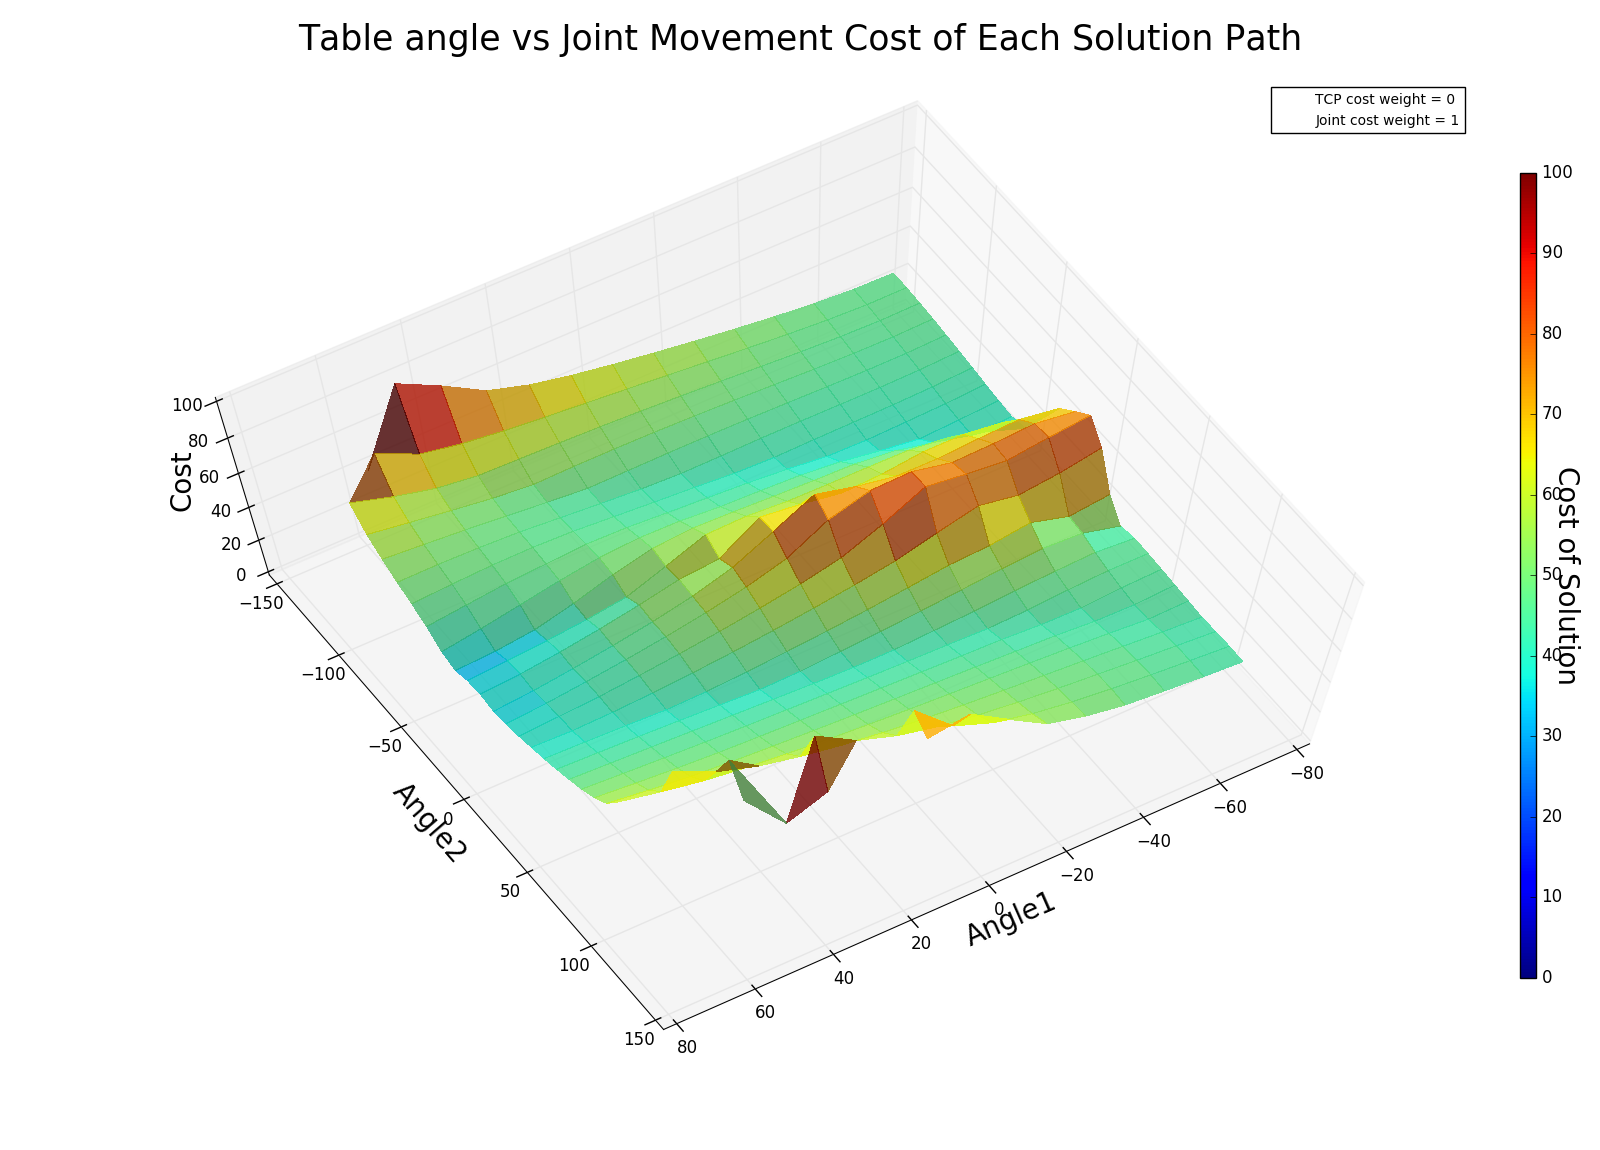
\includegraphics[width=1\textwidth,height=0.2\textheight]{images/orihori_jntcst.png}}
		\caption{Cost Function Plot}  
		\label{fig:17b}
	\end{subfigure}	
	\begin{subfigure}[b]{0.4\textwidth}
		\frame{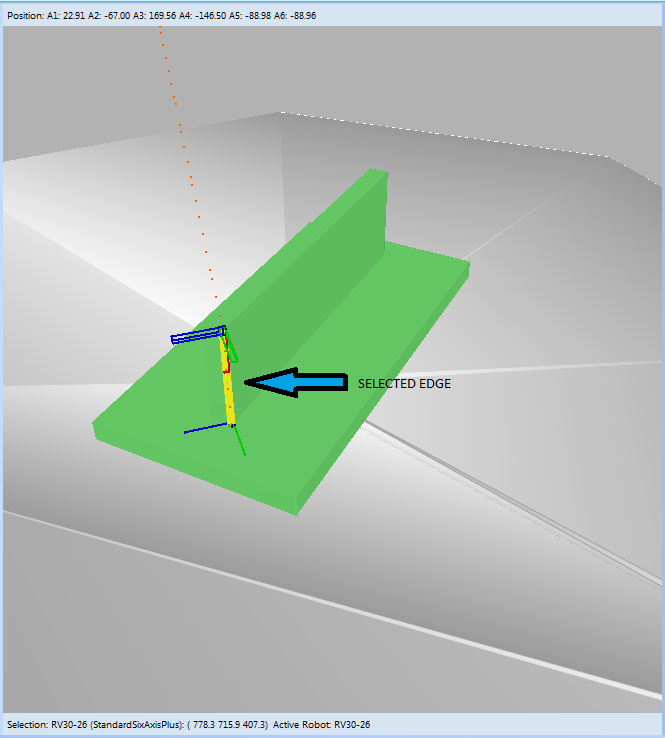
\includegraphics[width=1\textwidth,height=0.2\textheight]{images/normwp_left.png}}
		\caption{Edge to be welded}  
		\label{fig:17c}
	\end{subfigure}
	\begin{subfigure}[b]{0.4\textwidth}
		\frame{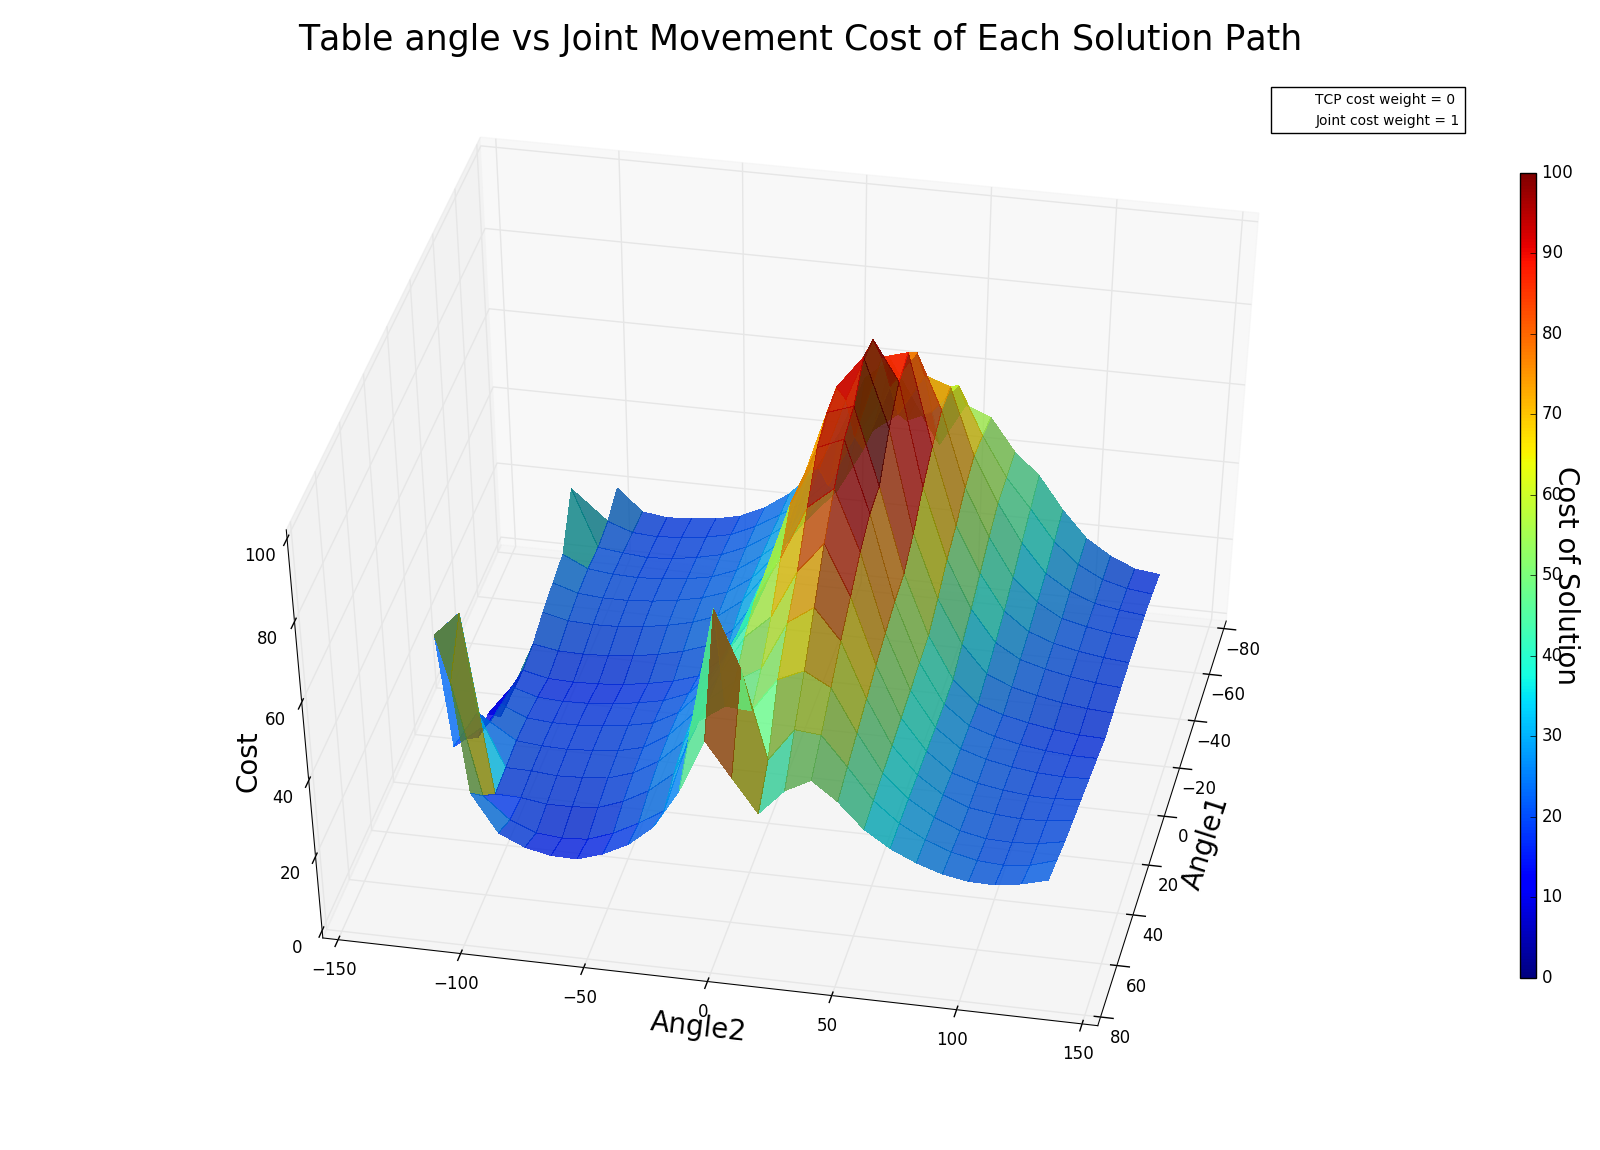
\includegraphics[width=1\textwidth,height=0.2\textheight]{images/orileft_jntcst2.png}}
		\caption{Cost Function Plot}  
		\label{fig:17d}
	\end{subfigure}	
	\caption{Cost Function Plot of T-Jointed workpiece: Joint Movement}
	\label{fig:17}
\end{figure}

From the plots (\ref{fig:17b}) \& (\ref{fig:17d}) of both the use cases, we can interpret that for the T-jointed workpiece, when both the joint angles of the table are at 0$^{\circ}$, the cost is the highest, which means for the weld paths at these positions of the table, the bigger joints move the most. While rotating  joint angle2 of the table has the most significant effect on generating solutions with lower cost. 
\clearpage

\begin{figure}[!ht] %  figure placement: here, top, bottom, or page
	\centering
	\begin{subfigure}[b]{0.4\textwidth}
		\frame{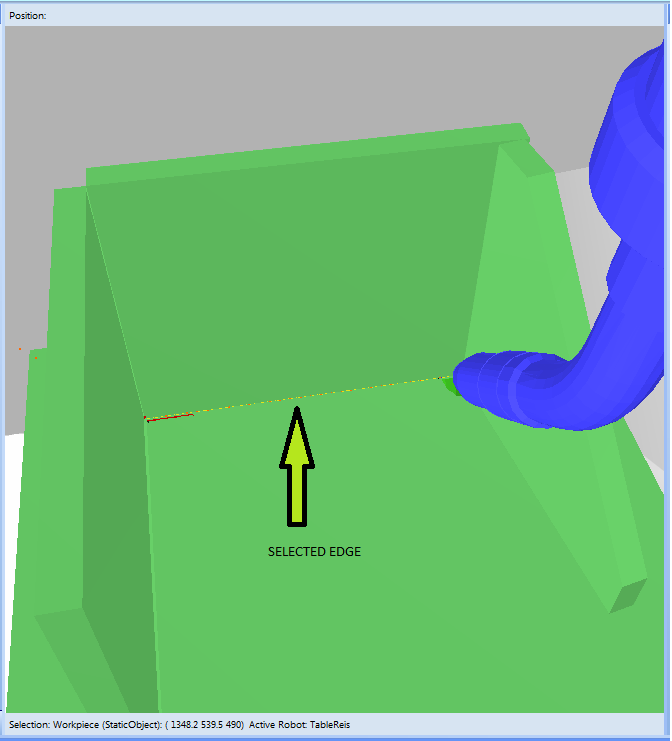
\includegraphics[width=1\textwidth,height=0.2\textheight]{images/auto_flat.png}}
		\caption{Edge to be welded}  
		\label{fig:18a}
	\end{subfigure}
	\begin{subfigure}[b]{0.4\textwidth}
		\frame{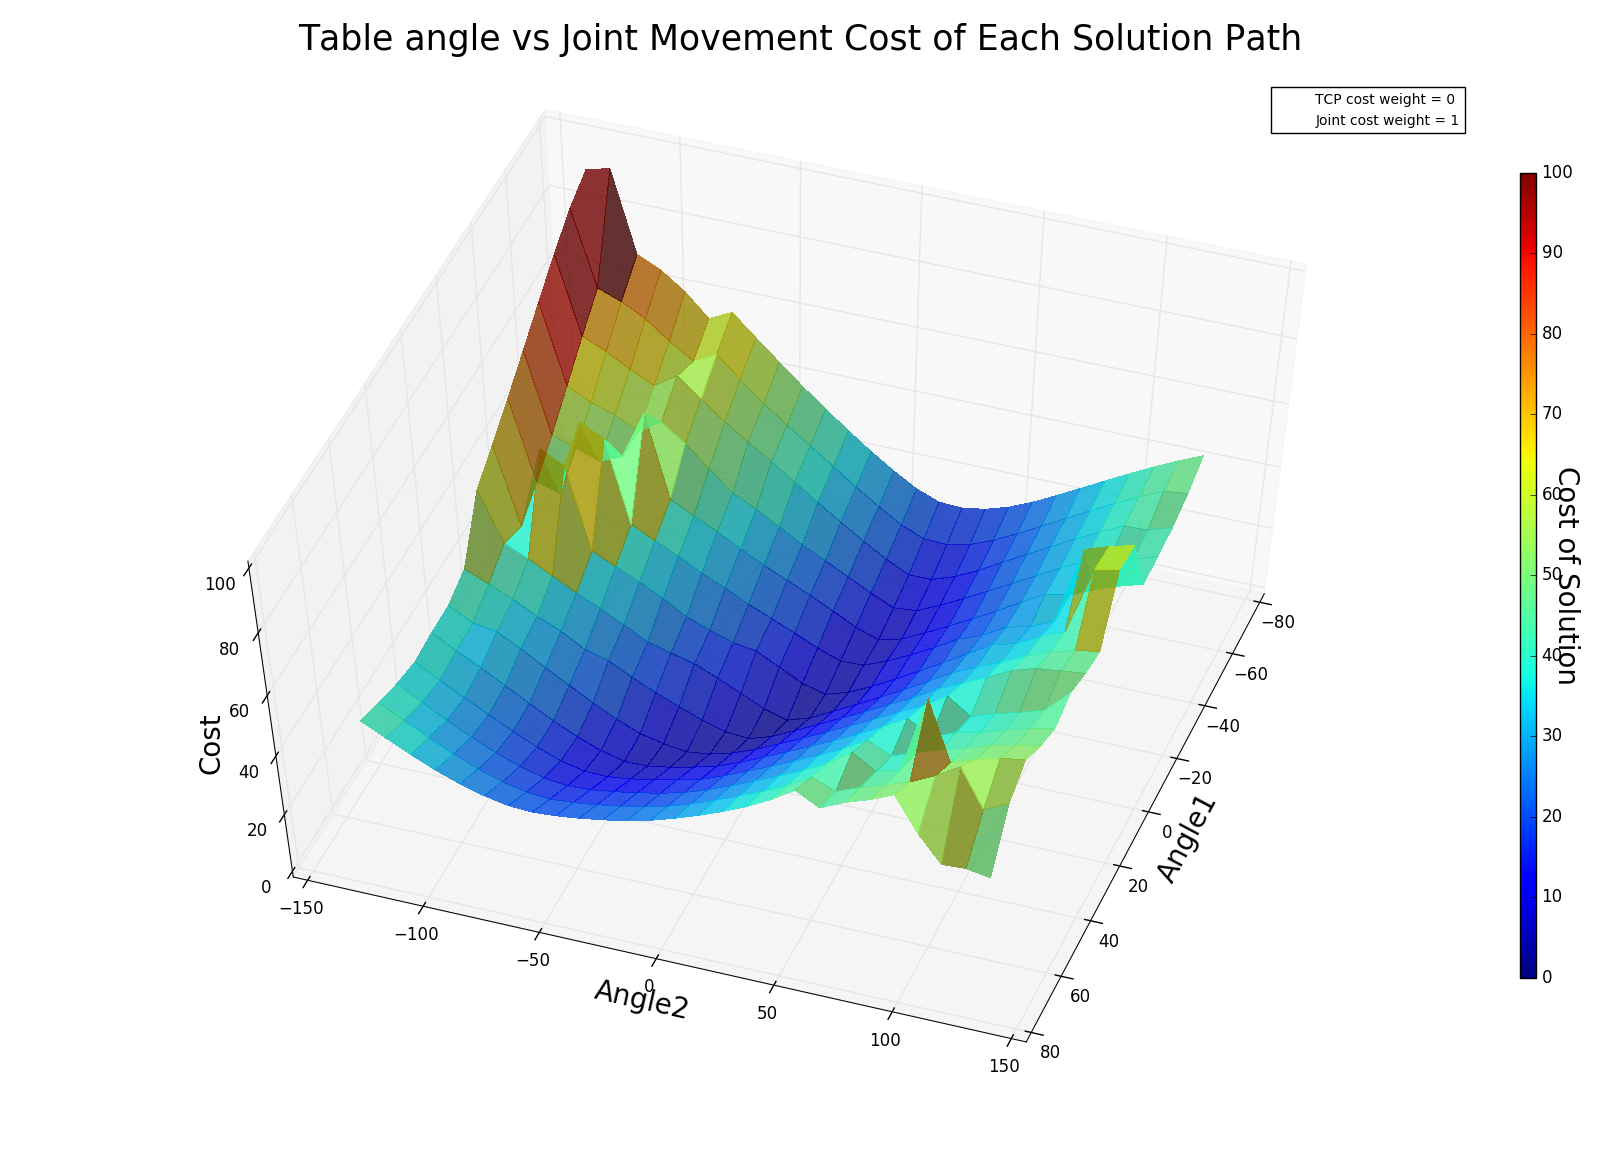
\includegraphics[width=1\textwidth,height=0.2\textheight]{images/autohori_jntcst.png}}
		\caption{Cost Function Plot}  
		\label{fig:18b}
	\end{subfigure}	
	\begin{subfigure}[b]{0.4\textwidth}
		\frame{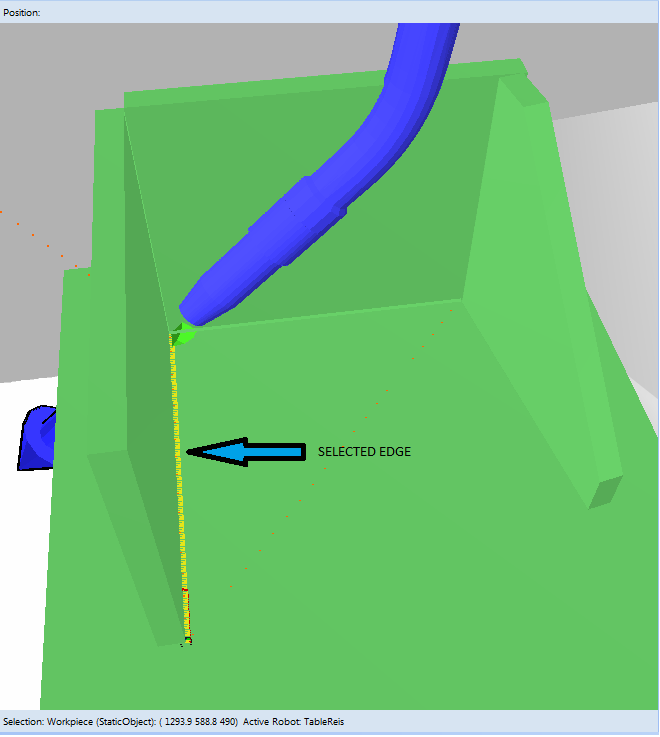
\includegraphics[width=1\textwidth,height=0.2\textheight]{images/auto_left.png}}
		\caption{Edge to be welded}  
		\label{fig:18c}
	\end{subfigure}
	\begin{subfigure}[b]{0.4\textwidth}
		\frame{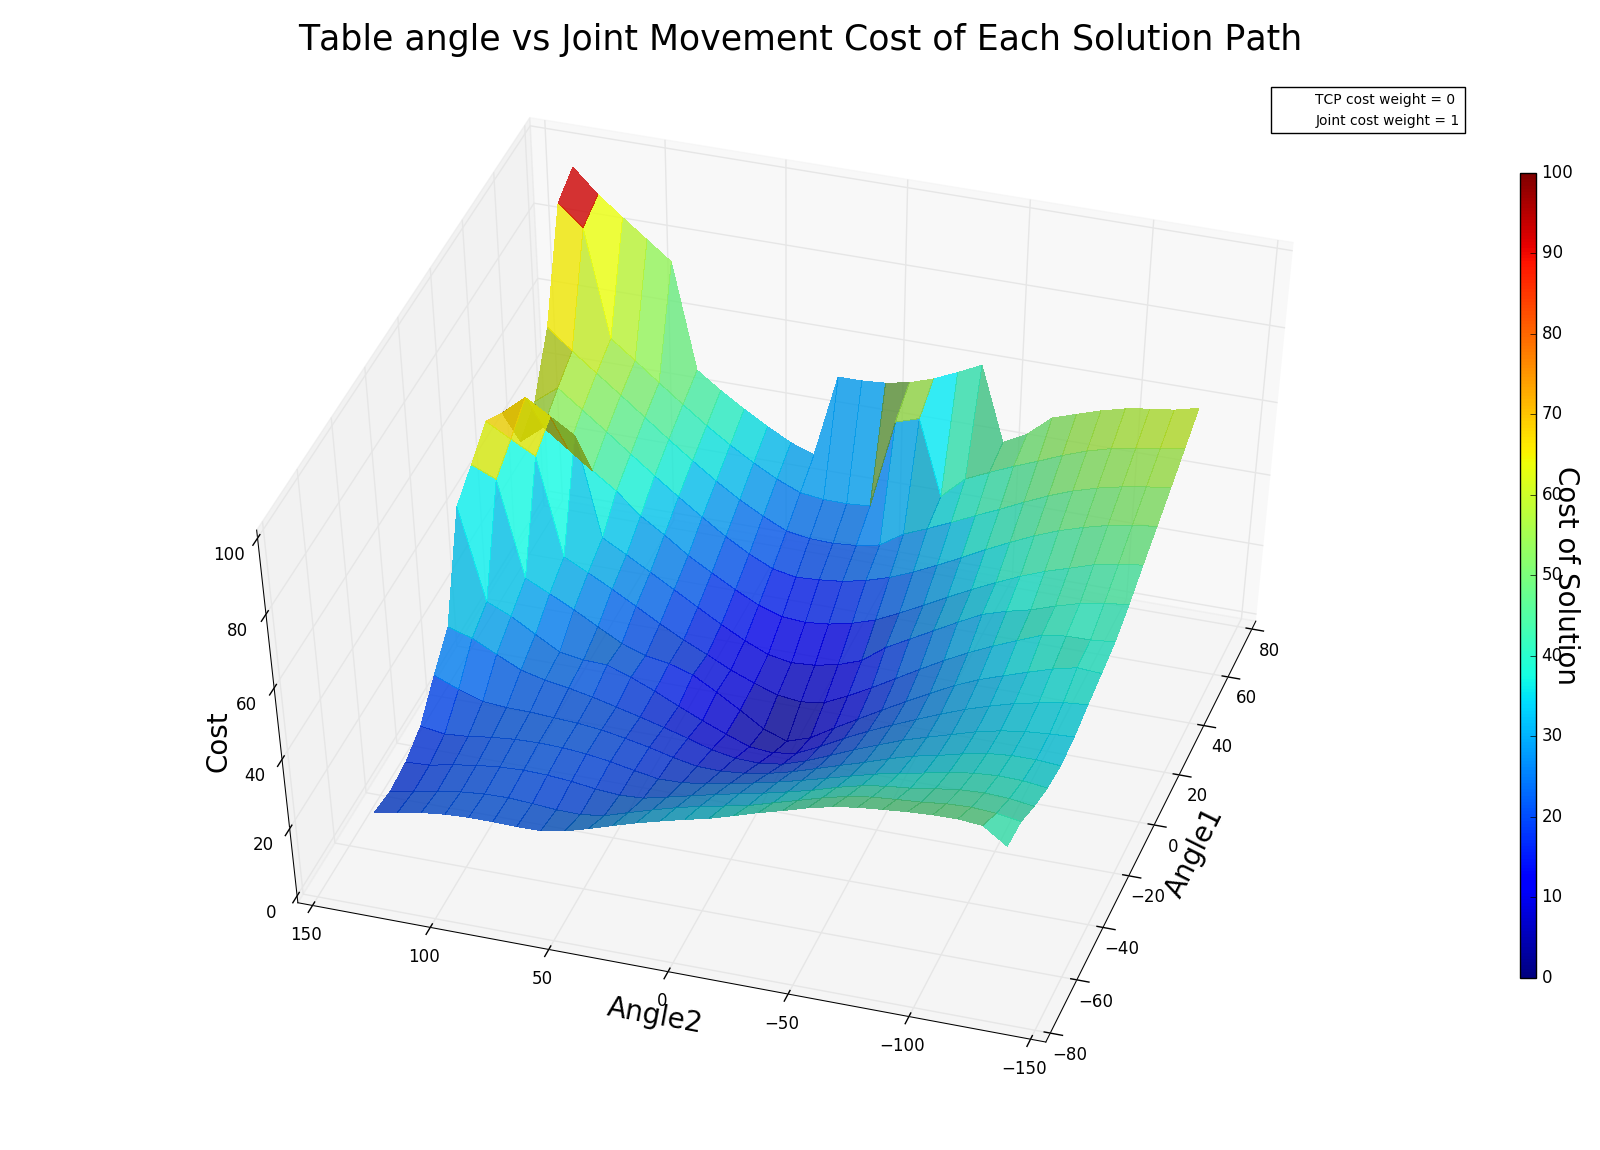
\includegraphics[width=1\textwidth,height=0.2\textheight]{images/autolft_jntcst.png}}
		\caption{Cost Function Plot}  
		\label{fig:18d}
	\end{subfigure}	
	\caption{Cost Function Plot of Automatica workpiece: Joint Movement}
	\label{fig:18}
\end{figure}

From the plots (\ref{fig:18b}) \& (\ref{fig:18d}) of both the use cases, we can interpret that for the Automatica workpiece, when both the joint angles of the table are at 0$^{\circ}$, the cost is the lowest, which means for the weld paths at these positions of the table, the bigger joints move the least, which is completely different from what we observed in (\ref{fig:17}). 

\subsubsection{Cumulative Cost Function}
Based on the cost functions defined in sections (\ref{sssec:tcpcst}) and (\ref{sssec:jntcst}), the cumulative cost function is formulated. The concept behind this cost function is that, based on the welding task and the environment in which it is to be performed we can decide which aspect of welding is more important. For e.g in cases where generating perfect welds are critical to the structural integrity of the end product, we can assign a greater weightage to the TCP orientation cost, as it is directly linked with the quality of weld based on process description as stated in (cite ppr). However a situation might also arise where consuming lesser power - while generating a weld path - is more relevant for e.g while prototyping an user will weld on a workpiece multiple times in which case his/her main priority would be minimize the power consumption instead of generating a perfect weld. The mathematical formulation of the cumulative cost function is presented in \ref{eq25}, where $C_{agg}$ is the cumulative sum, $w_{tcp}$ and $w_{joint}$ are the weights assigned to TCP and joint costs respectively and $C_{tcp}$ and $C_{joint}$ are the TCP and joint costs respectively. 
\begin{equation}
\label{eq25}
C_{agg}(\textit{Solution}) = w_{tcp}* C_{tcp} +  w_{joint}*C_{joint}
\end{equation}
Cumulative cost function plots for both use cases \hyperref[fig:uc1]{1} and \hyperref[fig:uc2]{2} were generated with the following weights: 
\begin{itemize}
\item TCP cost weightage:0.2, Joint cost weightage:0.8 
\item TCP cost weightage:0.4, Joint cost weightage:0.6
\item TCP cost weightage:0.5, Joint cost weightage:0.5
\item TCP cost weightage:0.6, Joint cost weightage:0.2
\end{itemize}

\begin{figure}[!ht] %  figure placement: here, top, bottom, or page
	\centering
		\frame{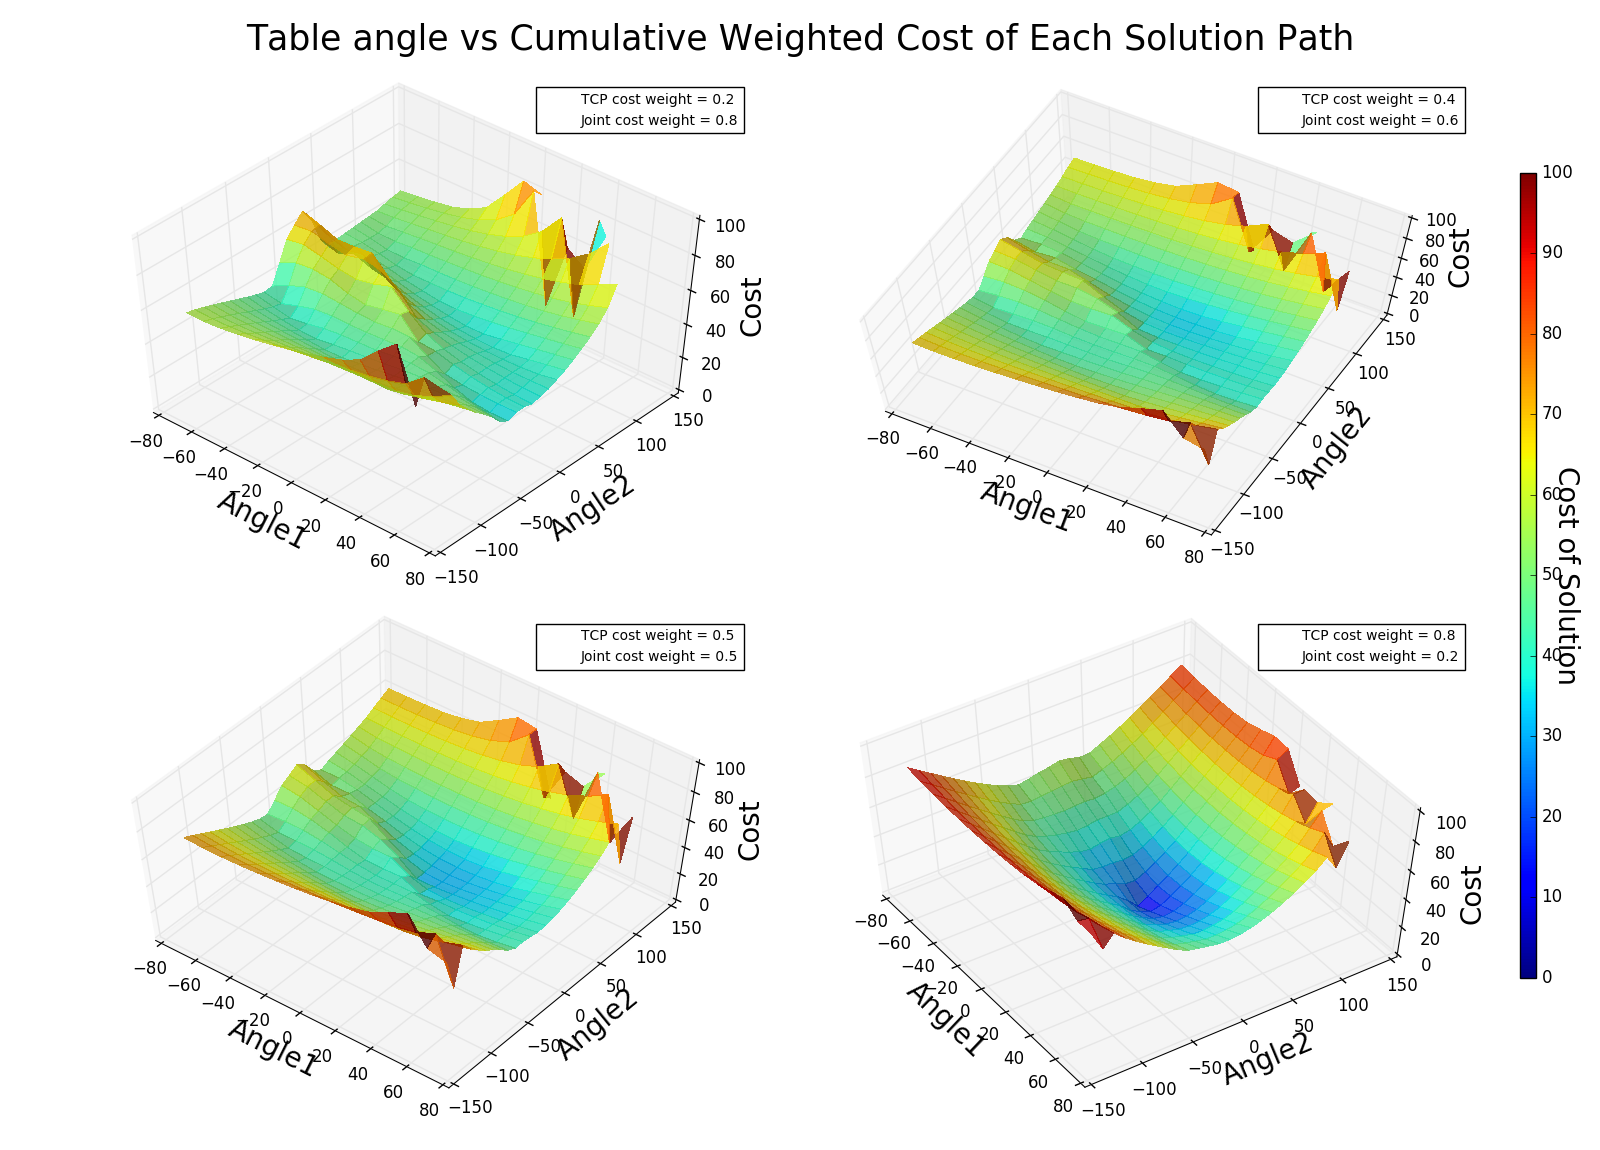
\includegraphics[width=1\textwidth]{images/orihori_totcst.png}}
		\caption{Cumulative Cost Function for T-Jointed Workpiece Horizontal Edge(\ref{fig:imguc1})}
		\label{fig:tot1}
\end{figure}
In plot \ref{fig:tot1}, we can observe that when the weightage values are both 0.5, a common area (marked by blue colored region), can be observed where the minimum cost of both the functions, overlap. For the other plots, the function with the higher weightage determines the shape of the plot, which is in accordance with our earlier results in sections (\ref{sssec:tcpcst}) and (\ref{sssec:jntcst})

\begin{figure}[!ht] %  figure placement: here, top, bottom, or page
	\centering
	\frame{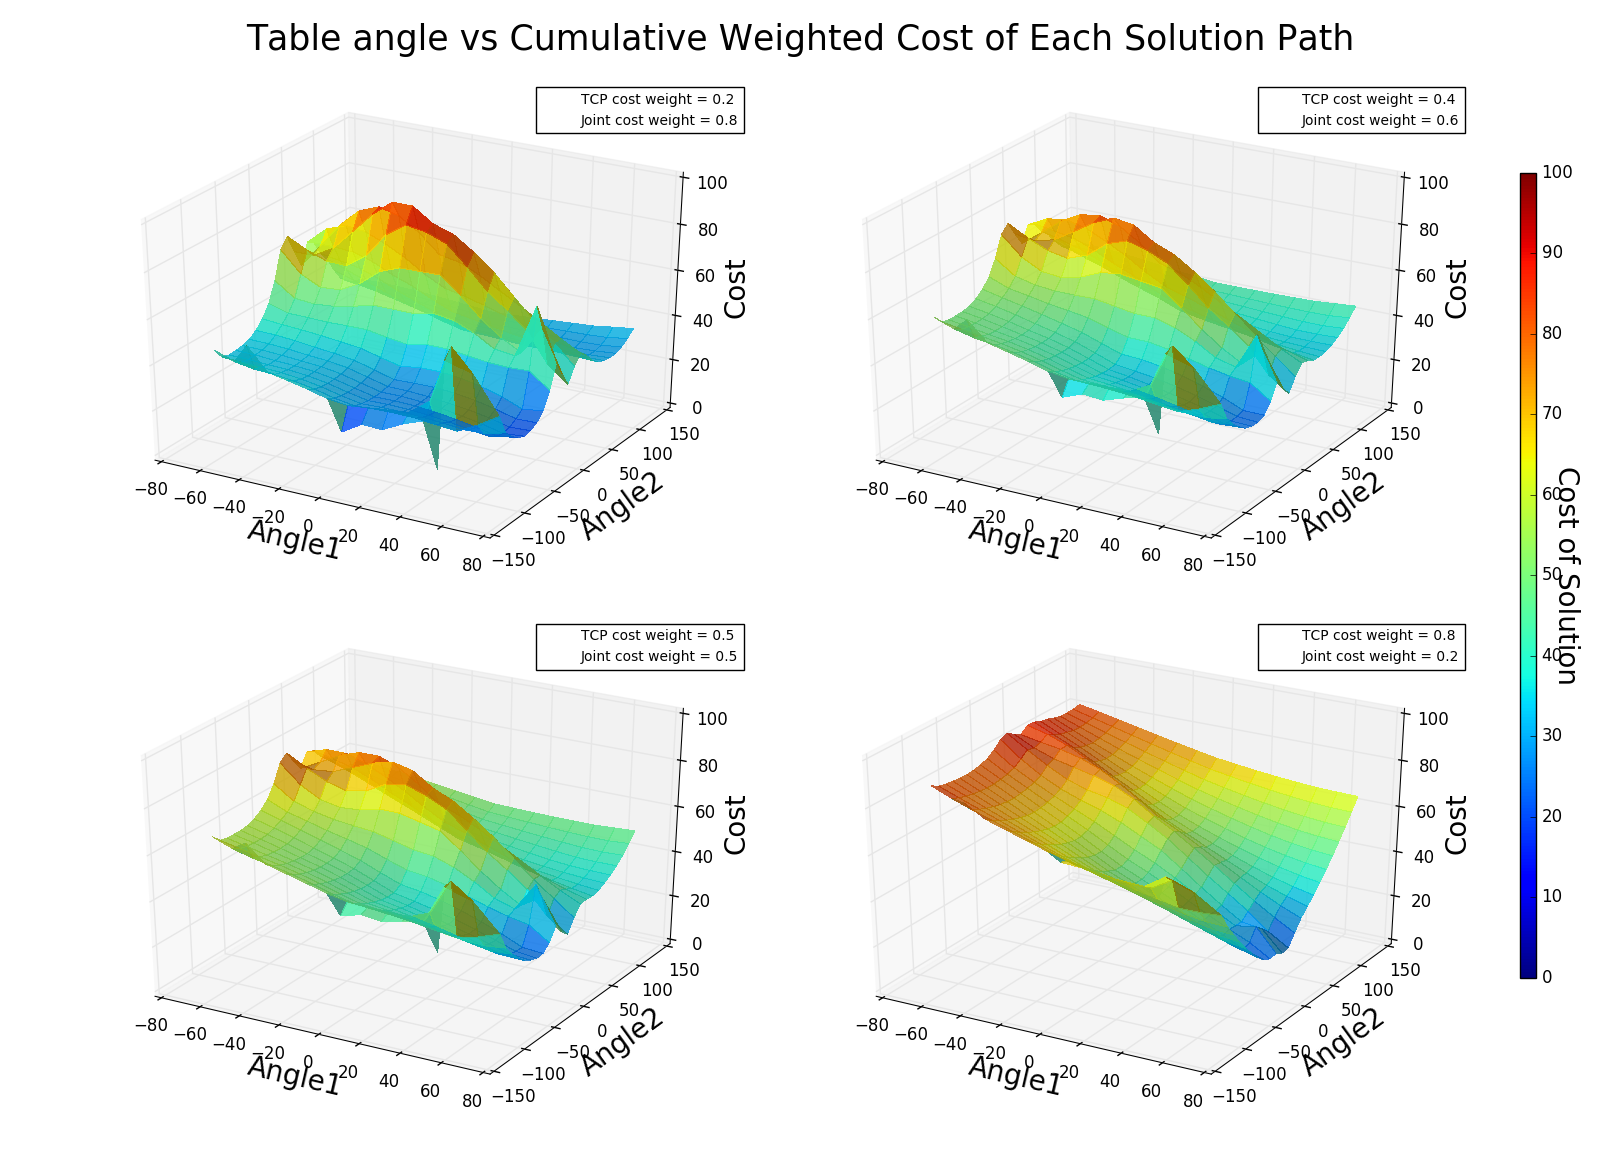
\includegraphics[width=1\textwidth]{images/orileft_totcst.png}}
	\caption{Cumulative Cost Function for T-Jointed Workpiece Vertical Edge(\ref{fig:imguc2})}
	\label{fig:tot2}
\end{figure}
Similarly in plot \ref{fig:tot2} we observe that, when the functions have equal weightage, a clear demarcation (marked by blue color) emerges. As in the previous case, the shape and features of the plot changes based on the weightage of the two functions. 

Next the plots for the \hyperref[fig:uc2]{2nd} use case are presented. 
\begin{figure}[!ht] %  figure placement: here, top, bottom, or page
	\centering
	\frame{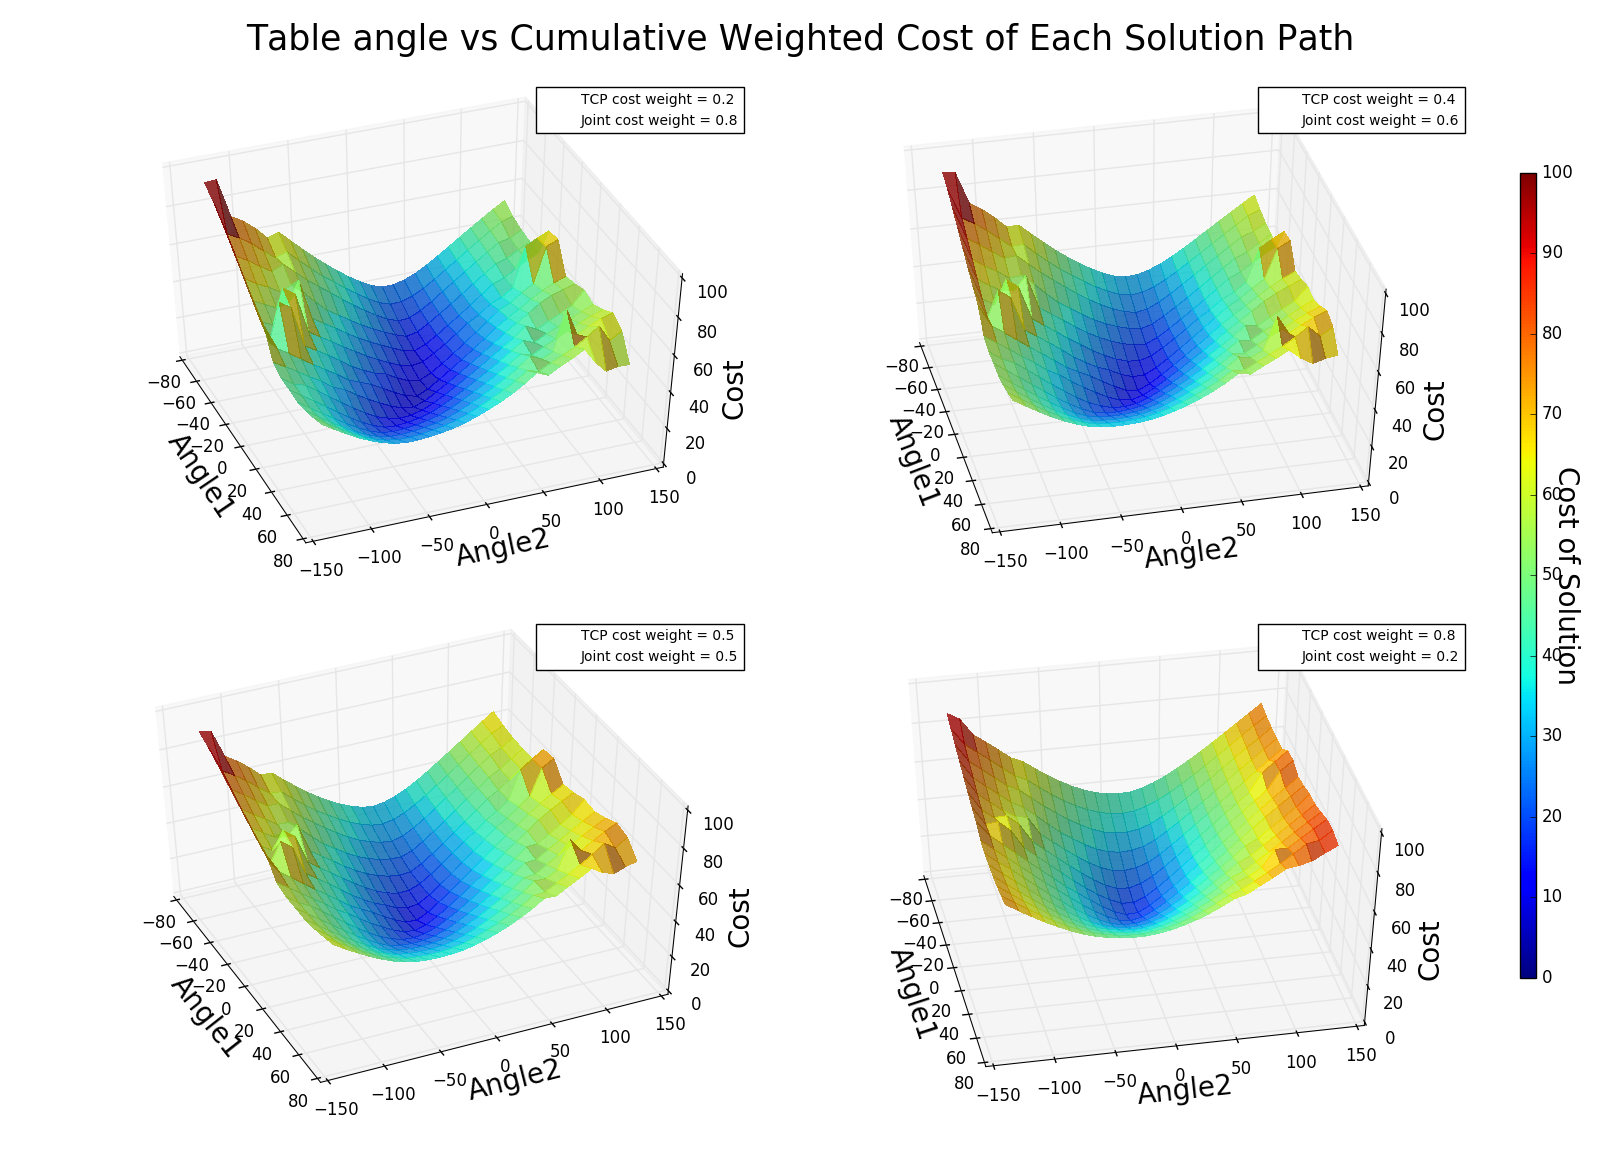
\includegraphics[width=0.8\textwidth,scale=0.6]{images/autohori_totcst.png}}
	\caption{Cumulative Cost Function for Automatica Workpiece Horizontal Edge(\ref{fig:imguc3})}
	\label{fig:tot3}
\end{figure}
Similarly in plot \ref{fig:tot3}, we can observe that when the weightage values are both 0.5, a common area (marked by blue colored region), can be observed where the minimum cost of both the functions, overlap. However for plot \ref{fig:tot4}, due to the fact the TCP cost for this use case is so high, it increases the overall minimum cost for the case when both the weightage values are 0.5. 

\begin{figure}[!ht] %  figure placement: here, top, bottom, or page
	\centering
	\frame{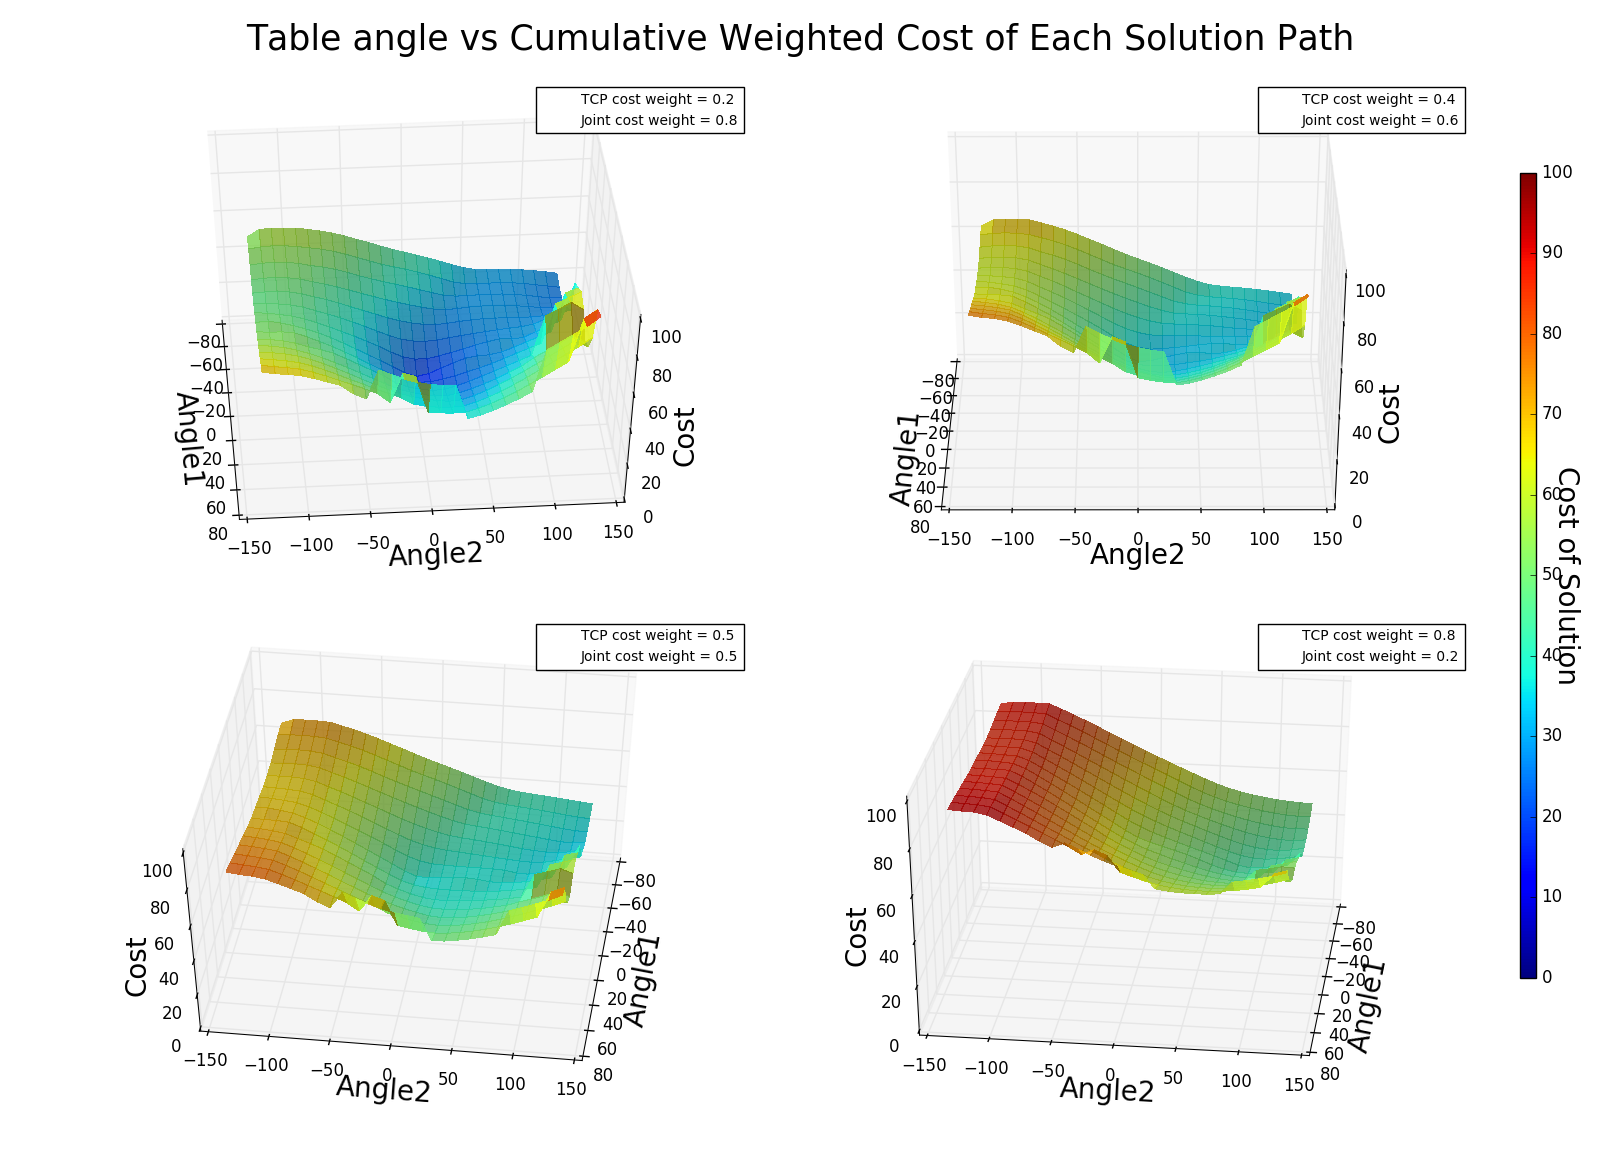
\includegraphics[width=0.8\textwidth,scale=0.6]{images/autolft_totcst.png}}
	\caption{Cumulative Cost Function for Automatica Left Horizontal Edge(\ref{fig:imguc4})}
	\label{fig:tot4}
\end{figure}
\clearpage

\subsection{Optimization Approaches}
(To determine min val)
In section \ref{ssec:cst} we plotted the cost functions for two use cases \ref{fig:uc1} and \ref{fig:uc2} and with the help of the plots we were able to determine for which values of the table joints, we can obtain weld paths with minimum cost. Even though this approach enables the user to see the cost space and make it very easy to select the optimal joint angles of the table, there are certain drawbacks to it:
\begin{itemize}
	\item The optimal cost value changes for every use case based on the workpiece, the edge to be selected and weightage of the TCP and joint cost functions.
	\item The difference in shape of the plots indicate, that it is also difficult to predict the cost values of a weld path just from the table angles, unless the solution is explicitly generated. 
	\item The inability to predict cost value coupled with the fact that the cost space is unique for different use cases, means that we have to generate plots for the entire range of the joint angles of the table for every welding use case.
	\item The generation of weld paths for every possible orientation of the table takes approximately 1 hour, which makes this process both tedious and inefficient. 
\end{itemize}
From the remarks, we can conclude that the problem at hand is a NP-hard problem, therefore the only possible way to find or approximate the optimal position would be to apply search based techniques. We consider two well known search algorithms - (i) Hill Climbing and (ii) Simulated Annealing - to find the optimum solution. While there are a plethora of other search based technique in use, for e.g Genetic/Evolutionary Algorithm - Hill Climbing or Simulated Annealing offer a perfect balance between finding the optimum and convergence time.
\subsubsection{Hill Descent Algorithm Approach}
\label{sssechd}
Hill Climbing or in our problem case, Hill Descent is a simple optimization technique which attempts to find new state from its current state by evaluating a cost function(cite russell norvig). Hill descent is based on a greedy approach, i.e. it only considers the subsequent state if it is locally optimal or in other words, if the cost value of the subsequent state is lower compared to the current state. Since it does not store the previous state values, it is extremely memory efficient and fast, which make it an ideal choice for our use case. A key consideration for the algorithm to function properly - in the use case at hand - is to determine the exit criteria. The simple reason being, because the global optimum value cannot be pre-determined, we can neither specify the exit criteria as a difference of current and next solution state nor can we fix the number of iterations, as in both the cases it might lead to a suboptimal solution. Since hill descent algorithm does not use any data structure to store already explored states, the following simple solution has been devised. 
\begin{itemize}
	\item Selection of new neighbors using Manhattan/Taxicab Distance (cite paper).
	\item This limits the number of possible neighbors to 8 for each state, since the we have a 2D space. 
	\item Following the above two conditions, we can assume that if for a certain state, all of its neighbors have higher cost values, that state can be considered as an optimum and the algorithm is terminated.
\end{itemize}

\algdef{SE}[DOWHILE]{Do}{doWhile}{\algorithmicdo}[1]{\algorithmicwhile\ #1}%
	
\begin{algorithm}
	\caption{Hill Descent Approach for Optimal Weld Path Generation}
	\label{algo4}
	\textbf{Given:} $ \text{Initial table joint angle values \textit{$A1$} \& \textit{$A2$}}$ \\ 
	\textbf{Output:} $ \text{Table joint values for plan path generation with minimum cost}$ \\
	
	\begin{algorithmic}[1]
		\State $\text{Apply kinematic equation \ref{eq22} and set table position using \textit{$A1$} \& \textit{$A2$}}$
		\State $\text{Apply Workpiece Transformation Algorithm(\ref{algo2})}$
		\State $\text{Apply Selected Edge Transformation Algorithm(\ref{algo3})}$
		\State $\text{Perform Motion Planning on the transformed plan path and get \textit{Solution}}$
		\State $\text{\textit{CurrentCost} $\gets$ $C_{agg}$(\textit{Solution}) using equation\ref{eq25}}$
		\State $\text{(\textit{$A1_{curr}$},\textit{$A2_{curr}$}) $\gets$ (\textit{$A1$}, \textit{$A2$})}$
		\Do
		\State $\text{(\textit{$A1_{new}$},\textit{$A2_{new}$})}$ $\gets$ $\text{\textit{SelectNeighbor}(\textit{$A1_{curr}$},\textit{$A2_{curr}$},\textit{stepsize})}$
		\State $\text{Apply steps \textit{1-4} with (\textit{$A1_{new}$},\textit{$A2_{new}$})}$
		\State $\text{\textit{Stepcost} $\gets$ $C_{agg}$(\textit{Solution}) \ref{eq25}}$
		\State $\text{\textit{diff} $\gets$ \textit{Stepcost} - \textit{CurrentCost}}$
		\If {[${diff < 0}$]}
		\State $\text{\textit{PossibleMinimaCounter} $\gets$ 0}$
		\State $\text{(\textit{$A1_{curr}$},\textit{$A2_{curr}$}) $\gets$ (\textit{$A1_{new}$}, \textit{$A2_{new}$})}$
		\State $\text{\textit{CurrentCost} $\gets$ \textit{Stepcost}}$
		\Else
		\State $\text{increase \textit{PossibleMinimaCounter} by 1}$
		\EndIf  
		
		\doWhile{$\textit{PossibleMinimaCounter}$ $\leq$ 8}
		\State $\textit{return}$ ($\textit{$A1_{curr}$}$,$\textit{$A2_{curr}$}$)     
	\end{algorithmic}
\end{algorithm}
In algorithm \ref{algo4}, we randomly choose a new neighbor, using Manhattan Distance and if the new state has a lower cost, then it moves to the new state and the \textit{PossibleMinimaCounter} is set to zero. If however, the new neighbor has a higher cost value, then the \textit{PossibleMinimaCounter} is incremented by 1. If the value of \textit{PossibleMinimaCounter} reaches 8, then we consider that state as a minimum state and exit the algorithm. Following this, we execute the algorithm and plot the results.
\begin{figure}[!ht] %  figure placement: here, top, bottom, or page
	\centering
	\frame{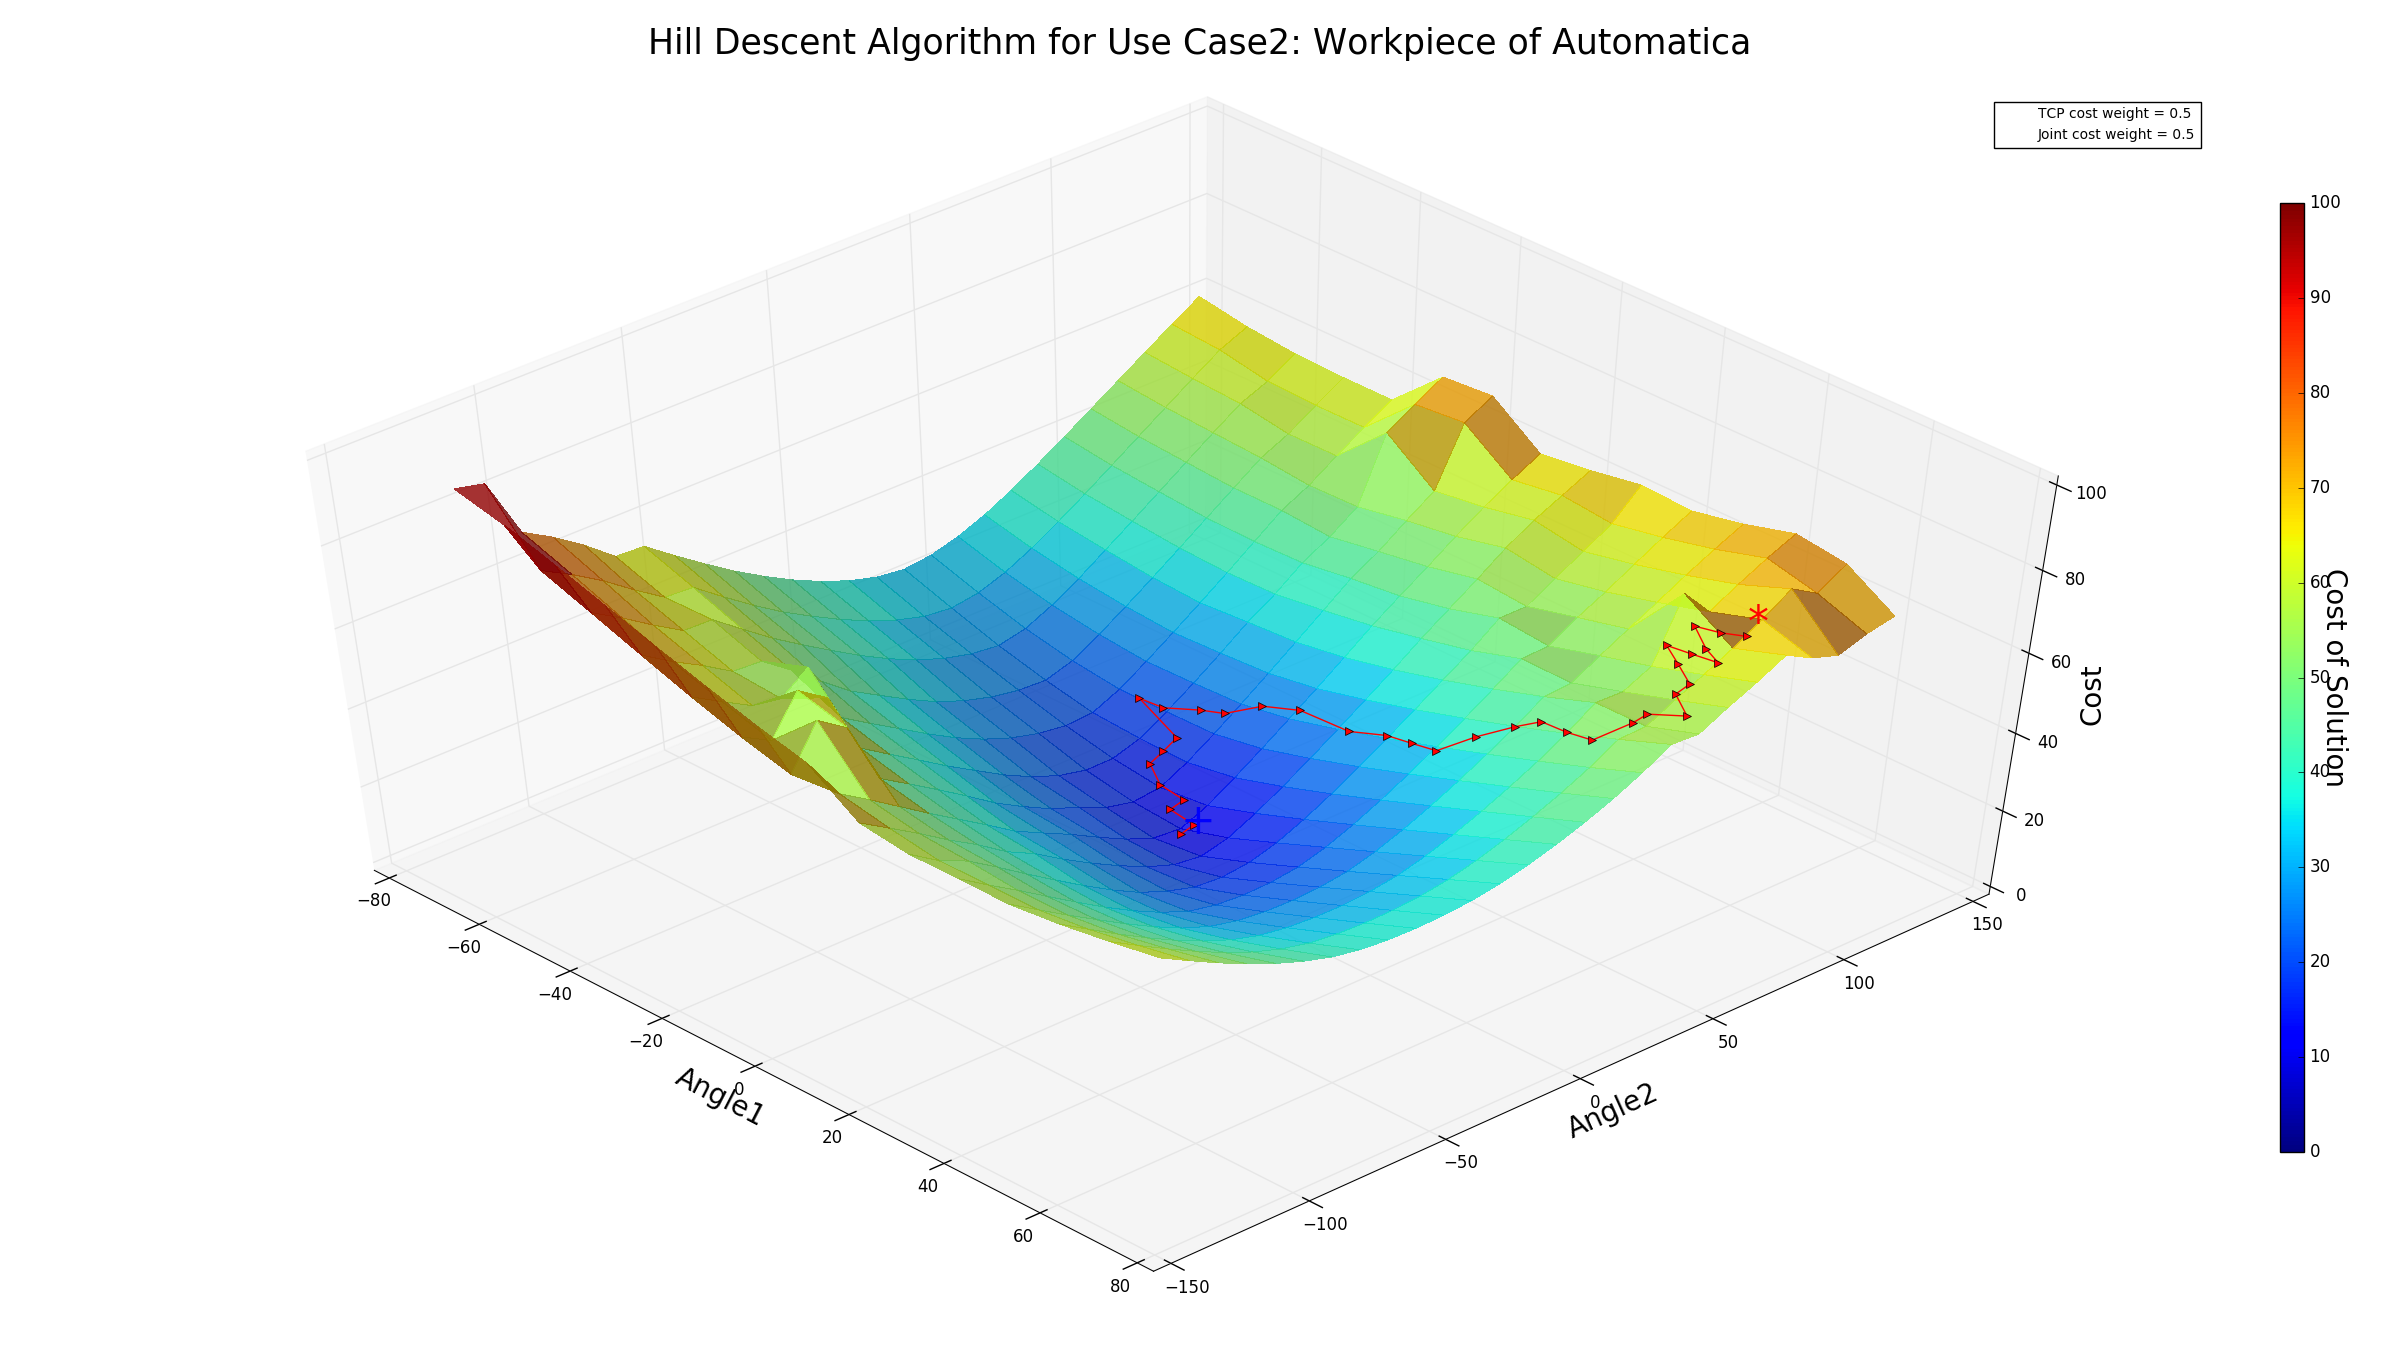
\includegraphics[width=0.8\textwidth,scale=0.6]{images/auto_hori_succ.png}}
	\caption{Hill Descent Optimization for Automatica Workpiece Horizontal Edge(\ref{fig:imguc3})}
	\label{fig:HD1}
\end{figure}
In figure \ref{fig:HD1}, the start state is marked by red star and the goal by blue plus. We can observe that, because the cost surface has a single global minimum, the hill descent approach was able to reach the global minima state.
\begin{figure}[!ht] %  figure placement: here, top, bottom, or page
	\centering
	\frame{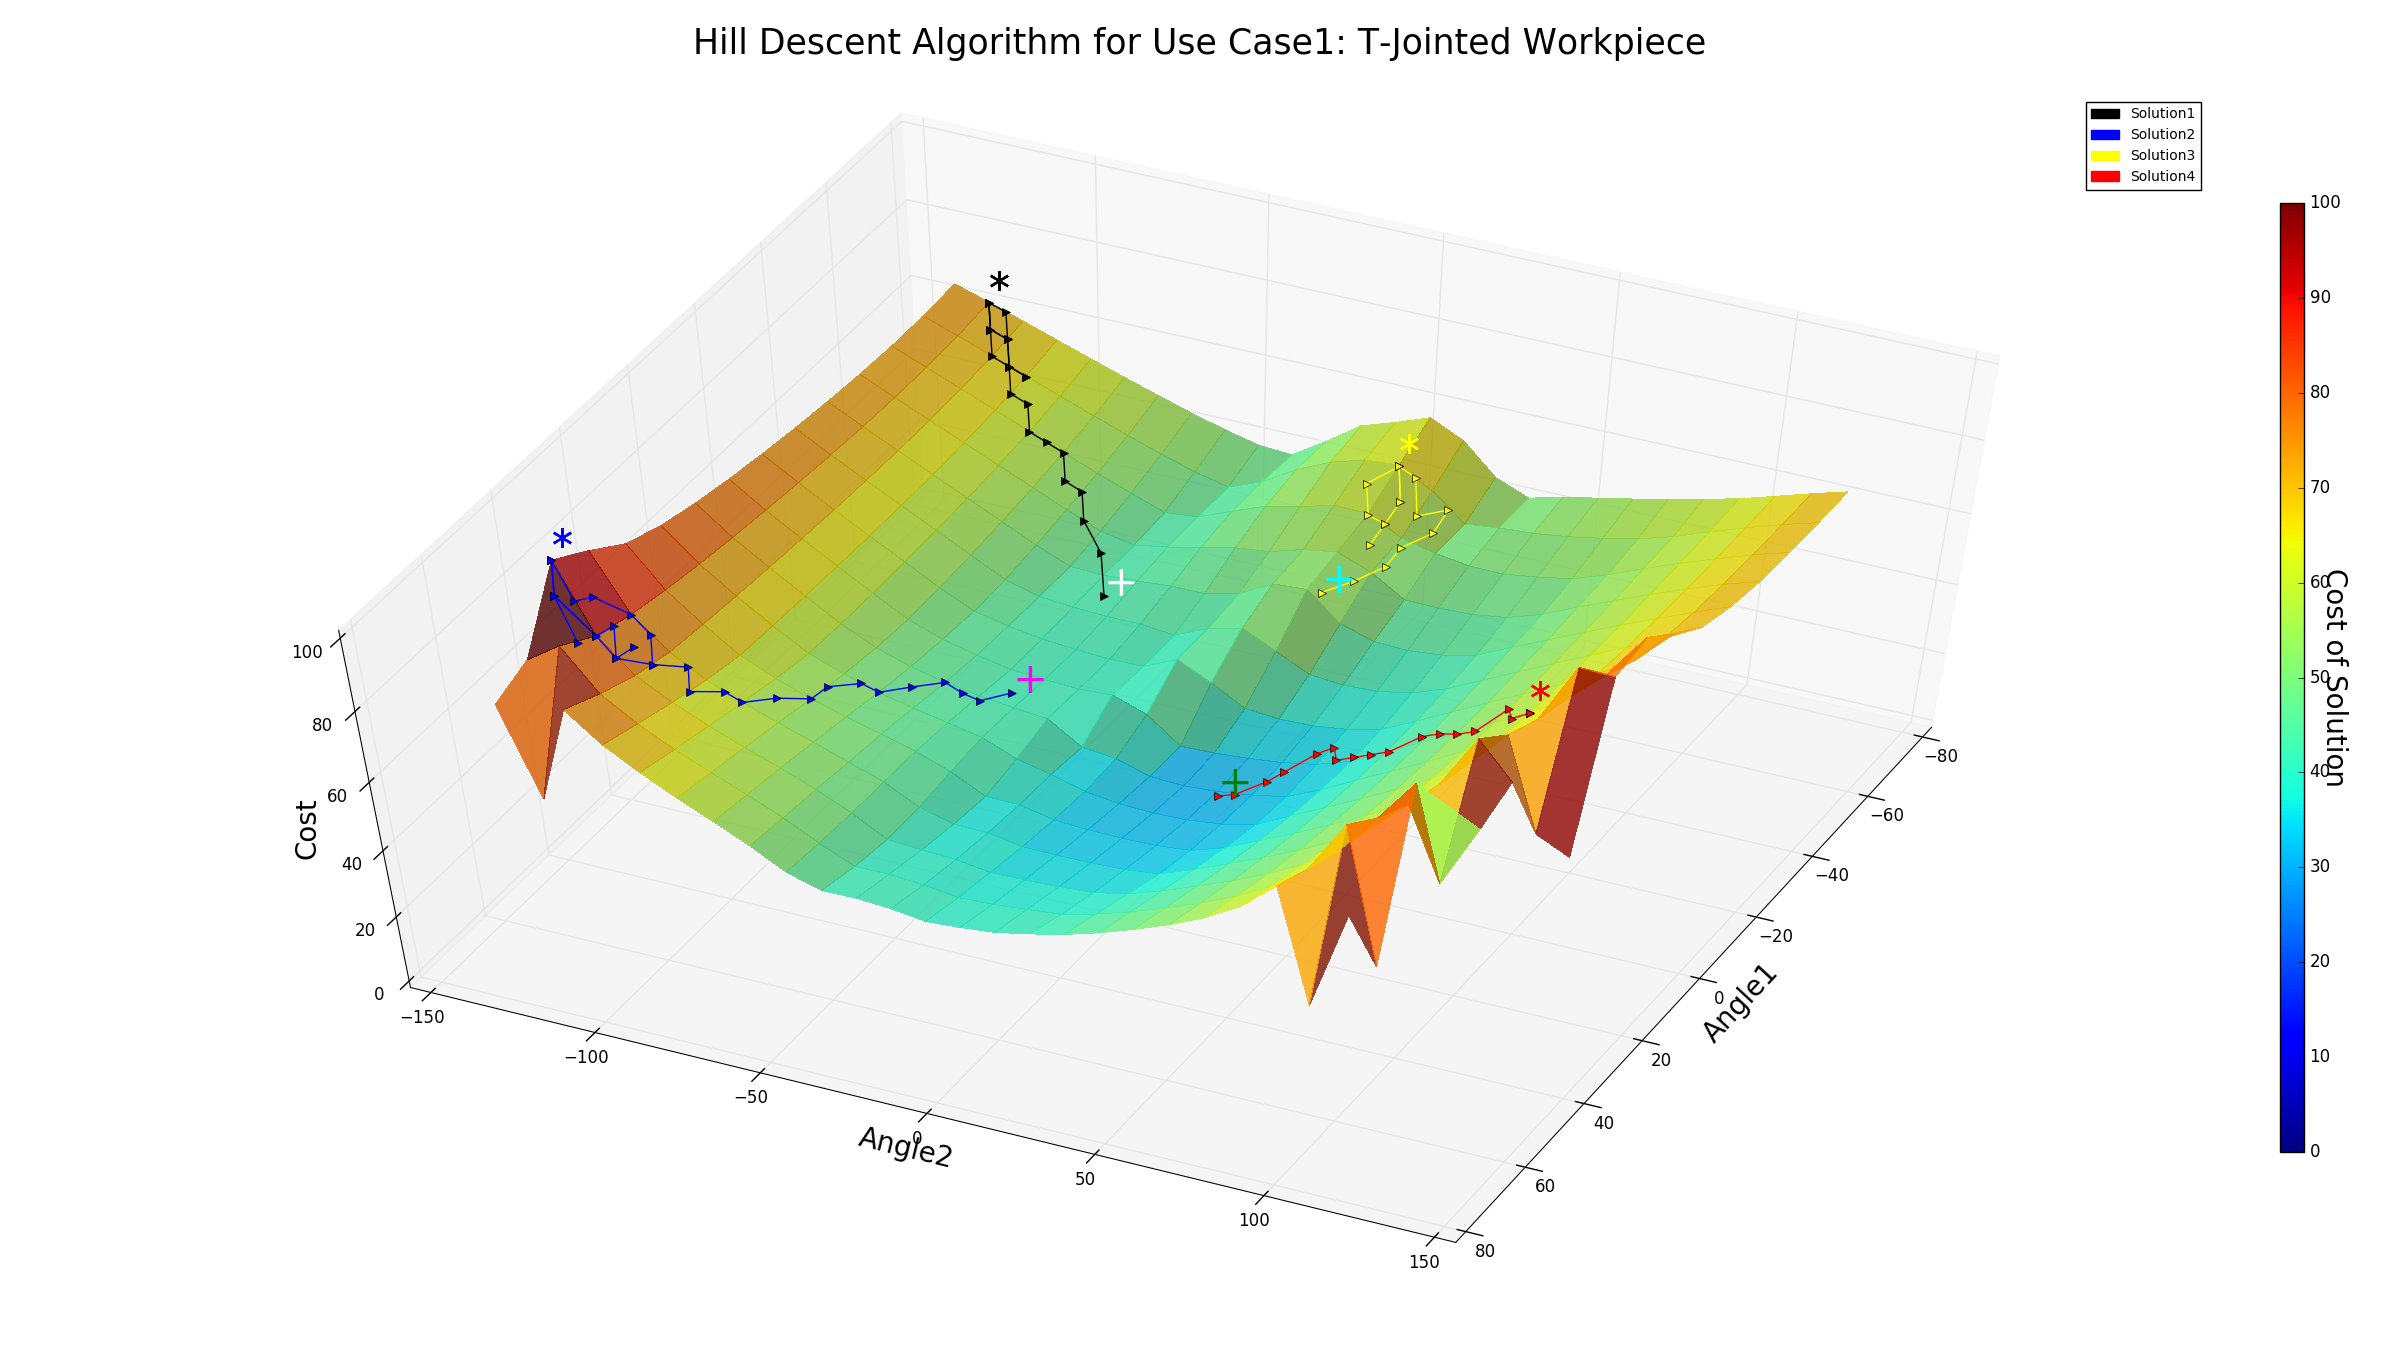
\includegraphics[width=0.8\textwidth,scale=0.6]{images/ori_hill_fail.png}}
	\caption{Hill Descent Optimization for T-Jointed Workpiece Horizontal Edge(\ref{fig:imguc2})}
	\label{fig:HD2}
\end{figure}\\
However, in figure \ref{fig:HD2} we can see that, because the cost surface has multiple local minima, the Hill Descent based approach gets stuck in a local minima for solutions 1, 2 and 3. This is a well known disadvantage of Hill Descent Algorithm, which nullifies its advantages of low memory consumption and speed\footnote{\label{fn1}To be noted: In figure (\ref{fig:HD1}) and (\ref{fig:HD2}) the cost plots are only shown for illustrative purposes, in the actual program, only the final optimized solution is returned.}. 
\subsubsection{Simulated Annealing Algorithm Approach}
In \ref{sssechd}, we observed that the Hill Descent Approach fails to find the most optimal solution, if it encounters a local minima. Simulated Annealing is typically used for cases where the search space might contain one or more local minima points along with a global minima. Simulated annealing can escape local minima by accepting moves with higher cost, based on the outcome of a probability function (cite sa paper). 
\begin{algorithm}[!ht]
	\caption{Simulated Annealing Approach for Optimal Weld Path Generation}
	\label{algo5}
	\textbf{Given:} $ \text{Initial table joint angle values \textit{$A1$} \& \textit{$A2$}}$ \\ 
	\textbf{Output:} $ \text{Table joint values for plan path generation with minimum cost}$
	
	\begin{algorithmic}[1]
		\State $\text{Apply kinematic equation \ref{eq22} and set table position using \textit{$A1$} \& \textit{$A2$}}$
		\State $\text{Apply Workpiece Transformation Algorithm(\ref{algo2})}$
		\State $\text{Apply Selected Edge Transformation Algorithm(\ref{algo2})}$
		\State $\text{Perform Motion Planning on the transformed plan path and get \textit{Solution}}$
		\State $\text{\textit{CurrentCost} $\gets$ $C_{agg}$(\textit{Solution}) using equation(\ref{eq25})}$
		\State $\text{(\textit{$A1_{curr}$},\textit{$A2_{curr}$}) $\gets$ (\textit{$A1$}, \textit{$A2$})}$
		\While {[${temperature > \epsilon}$]}
		\State $\text{(\textit{$A1_{new}$},\textit{$A2_{new}$})}$ $\gets$ $\text{\textit{SelectNeighbor}(\textit{$A1_{curr}$},\textit{$A2_{curr}$})}$
		\State $\text{Apply steps \textit{1-4} with (\textit{$A1_{new}$},\textit{$A2_{new}$})}$
		\State $\text{\textit{Stepcost} $\gets$ $C_{agg}$(\textit{Solution}) \ref{eq25}}$
		\State $\text{\textit{diff} $\gets$ \textit{Stepcost} - \textit{CurrentCost}}$
		\If {[${diff < 0 } \textit{ or }$ $e^{-1*diff/temperature} >$  $Rand(0,1) $]}
		\State $\text{(\textit{$A1_{curr}$},\textit{$A2_{curr}$}) $\gets$ (\textit{$A1_{new}$}, \textit{$A2_{new}$})}$
		\State $\text{\textit{CurrentCost} $\gets$ \textit{Stepcost}}$
		\EndIf
		\State $\textit{temperature}$ $\gets$ $\textit{temperature*coolingrate}$
		\EndWhile %doWhile{$\textit{PossibleMinimaCounter} < 8$}
		\State $\textit{return} (\textit{$A1_{curr}$},\textit{$A2_{curr}$})$      
	\end{algorithmic}
\end{algorithm}\\
Similar to hill descent approach, simulated annealing accepts any next move which has a lower cost compared to the current one, however unlike hill descent it also accepts a fraction of moves to states with higher solution cost. The probability of accepting moves to states with higher cost is determined by a continuously decreasing temperature parameter. 
The algorithm terminates when the temperature becomes less than an $\epsilon$ value. In algorithm (\ref{algo5}) , the new table joint angles are selected using euclidean distance. The new states are also stored in a data structure to ensure no duplicate neighbors are generated.
\begin{figure}[!ht] %  figure placement: here, top, bottom, or page
	\centering
	\frame{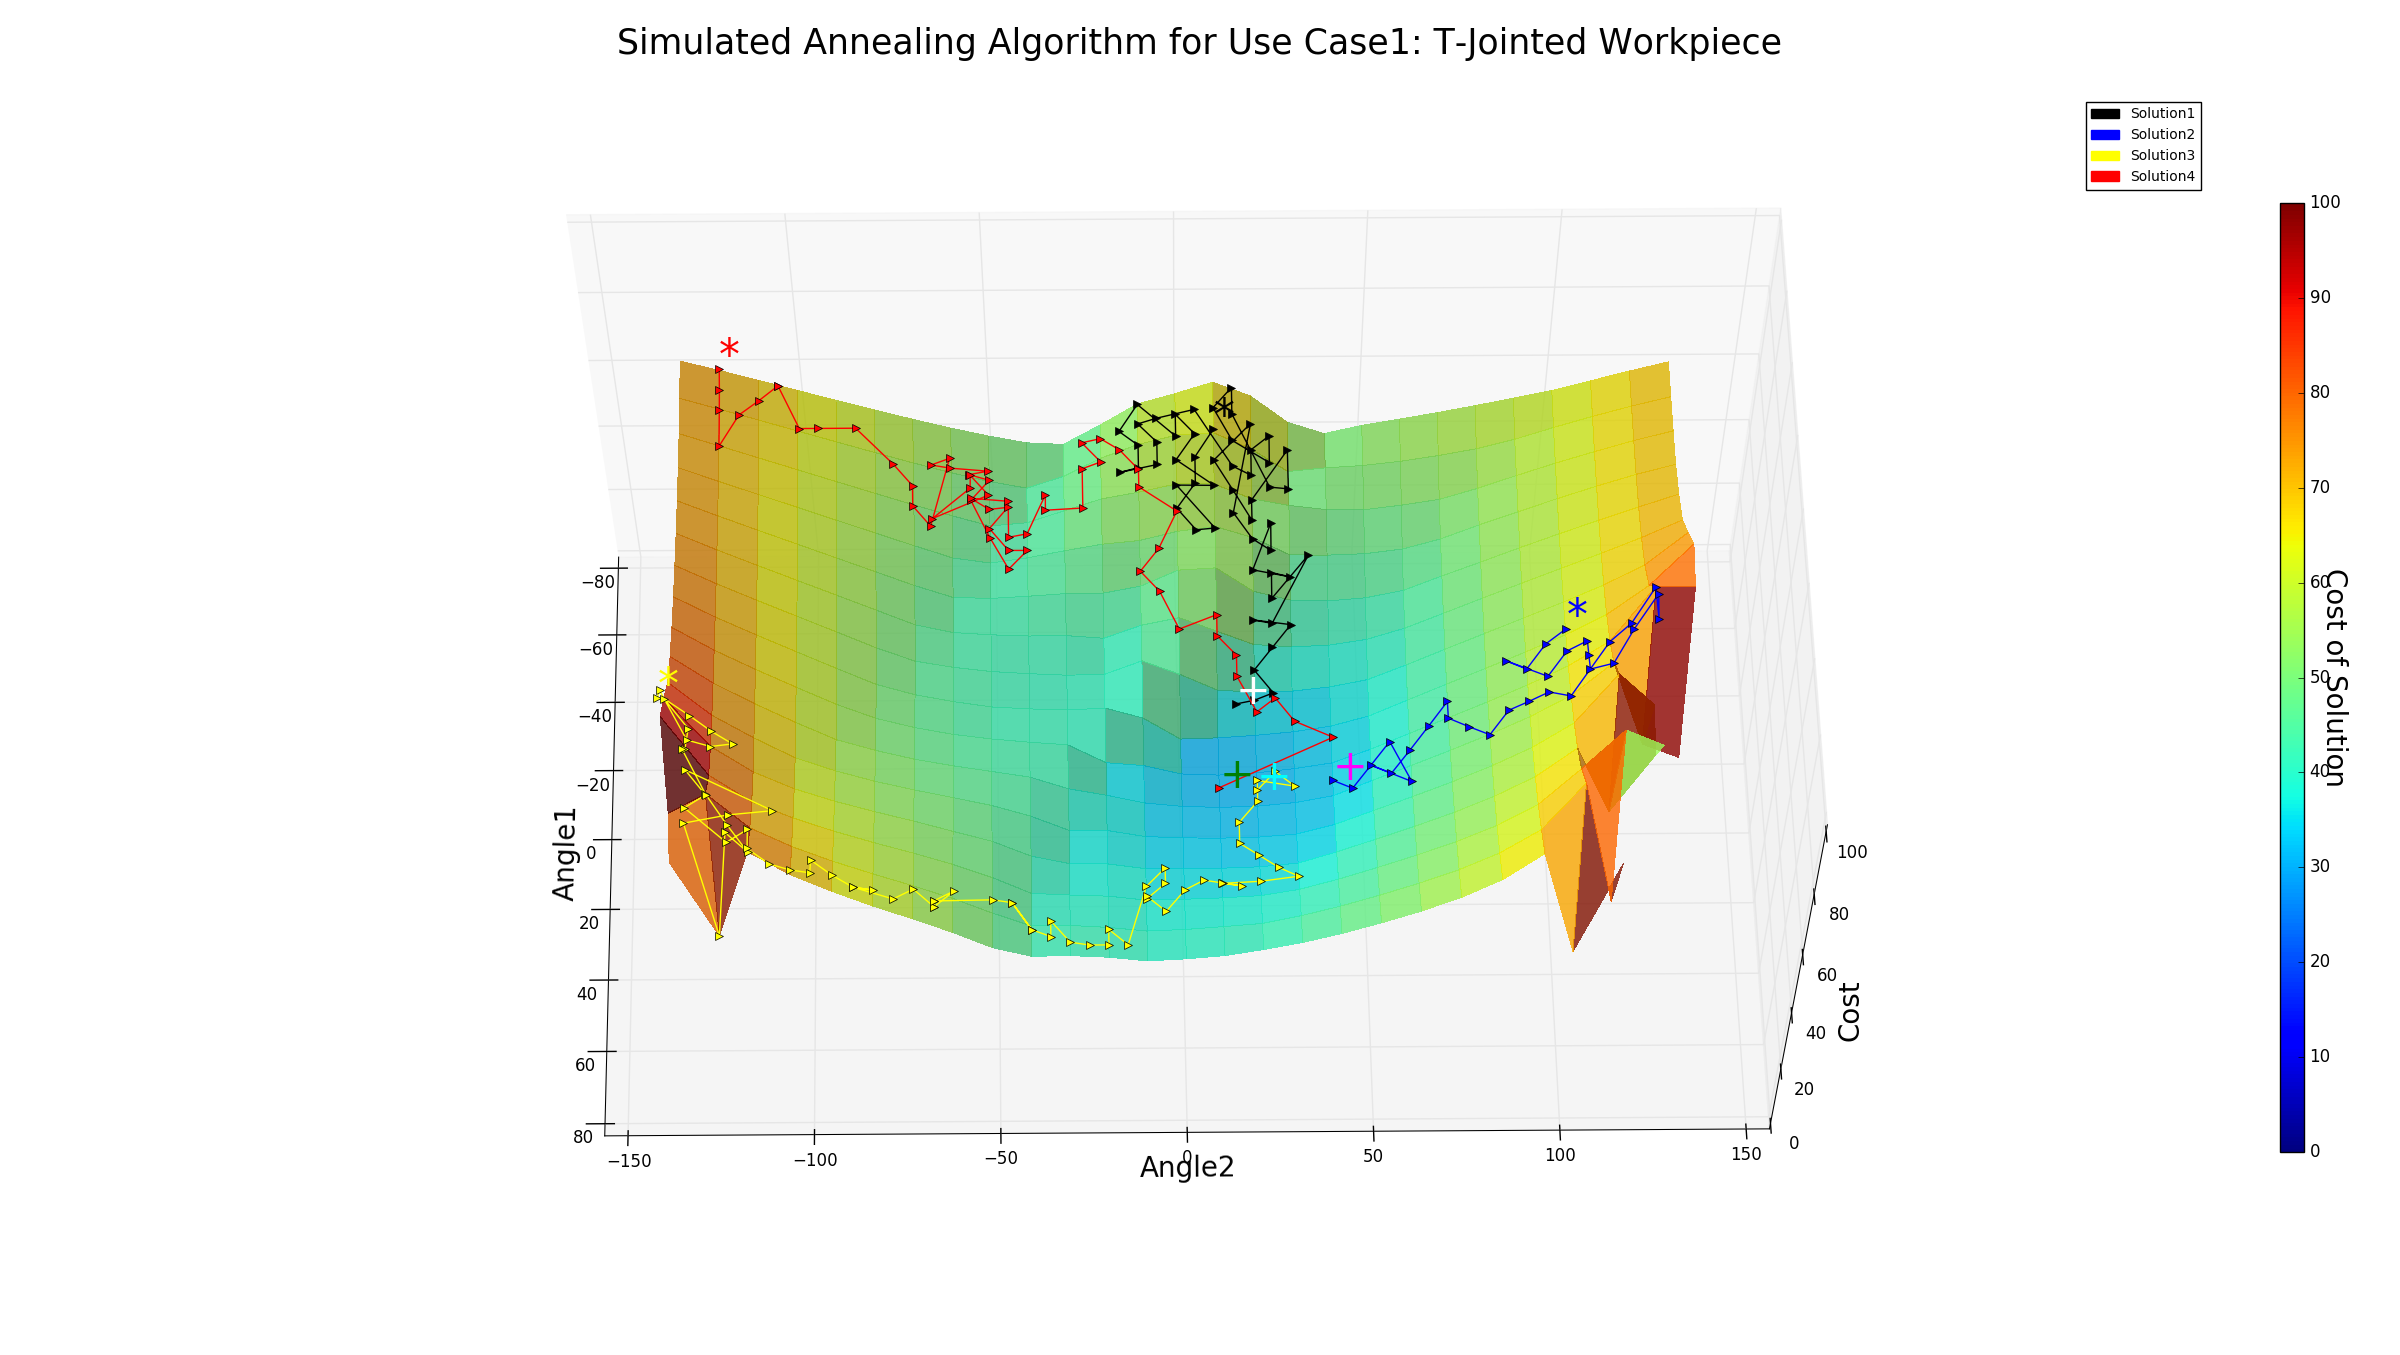
\includegraphics[width=0.8\textwidth,scale=0.6]{images/ori_sa_succ.png}}
	\caption{Simulated Annealing Optimization for T-Jointed Workpiece Horizontal Edge(\ref{fig:imguc2})}
	\label{fig:SA1}
\end{figure}
\begin{figure}[!ht] %  figure placement: here, top, bottom, or page
	\centering
	\frame{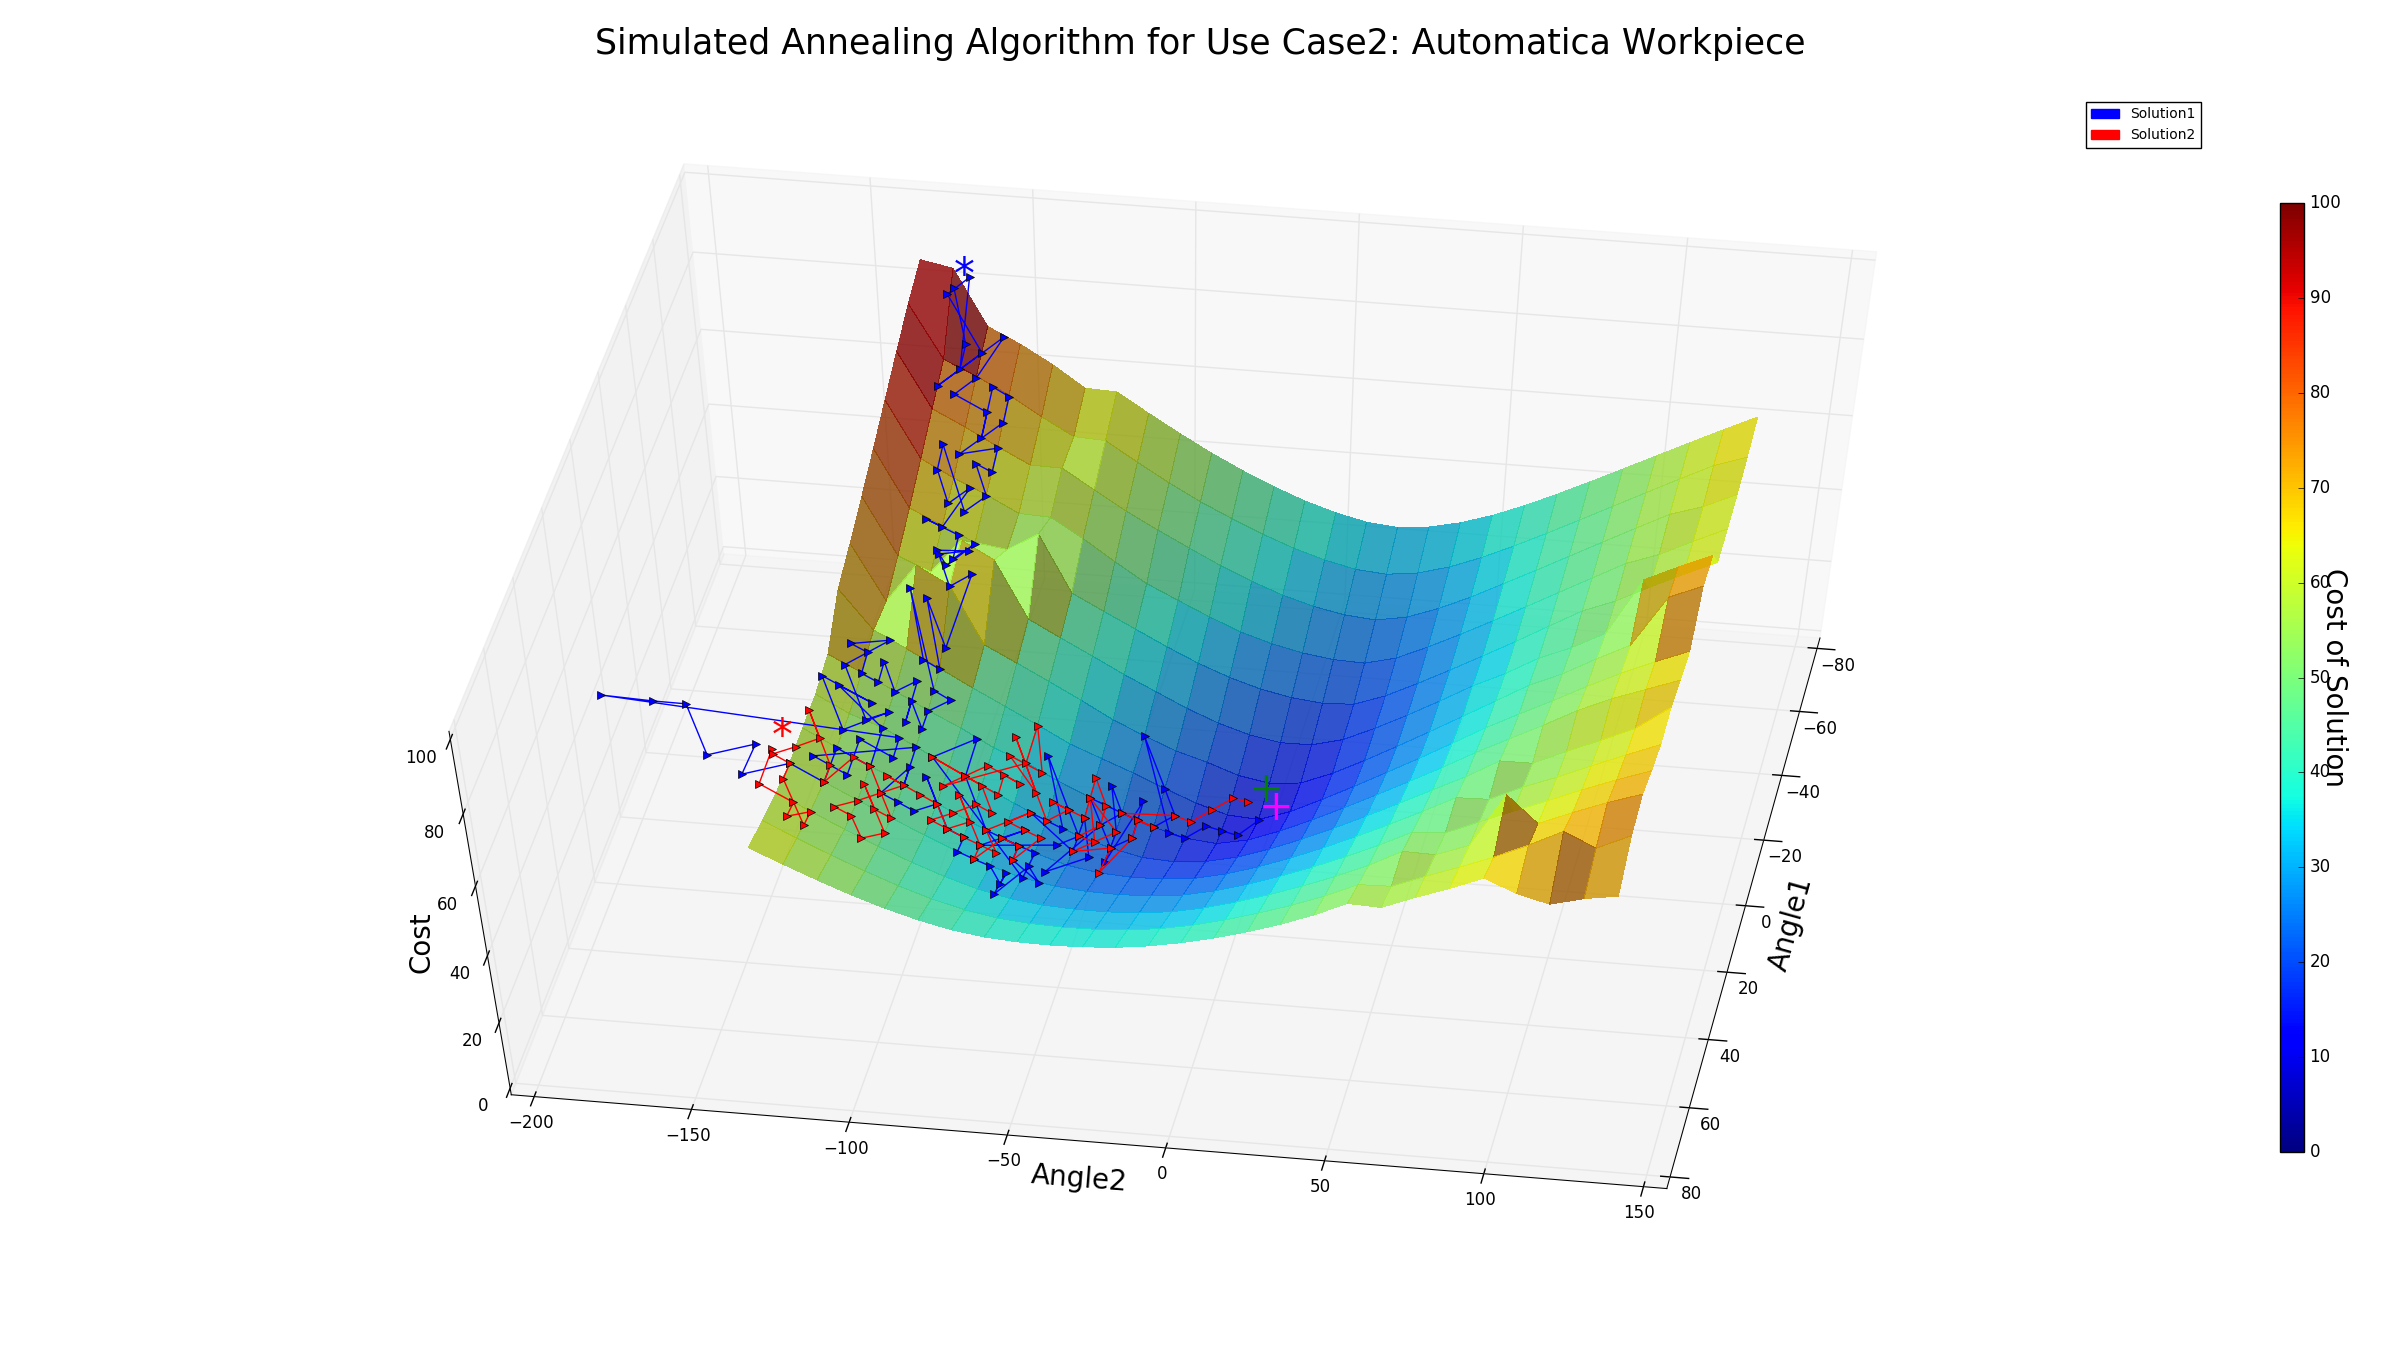
\includegraphics[width=0.8\textwidth,scale=0.6]{images/auto_sa_succ.png}}
	\caption{Simulated Annealing Optimization for Automatica Workpiece Horizontal Edge(\ref{fig:imguc3})}
	\label{fig:SA2}
\end{figure}\\
In figure \ref{fig:SA1} and \ref{fig:SA2}, the start and the goal states are  marked by '*' and '+' respectively. We can also observe that unlike the hill descent approach, it was able to find the optimal solution in all cases. However, unlike hill descent approach, in plot (\ref{fig:SA2}) it takes a lot more steps to reach the global minima state even when there are no local minima. 
\clearpage
\subsection{Comparative Evaluation and Analysis}












